% D7065E final report: architecture document for the Room Climate Control system.
% Build: see Makefile (pdflatex twice). Figures: diagrams/*.d2 -> figures/*.pdf.
\PassOptionsToPackage{unicode}{hyperref}
\PassOptionsToPackage{hyphens}{url}
\PassOptionsToPackage{dvipsnames,svgnames,x11names}{xcolor}
\documentclass[11pt]{article}
\usepackage{amsmath,amssymb}
\usepackage{lmodern}
\usepackage[T1]{fontenc}
\usepackage[utf8]{inputenc}
\usepackage{textcomp}
\usepackage[]{microtype}
\usepackage{parskip}
\usepackage{xcolor}
\usepackage{xurl}
\usepackage{bookmark}
\hypersetup{
  pdftitle={Room Climate Control, Architecture Document},
  pdfauthor={David Sämfors and Gustav Juul},
  colorlinks=true,
  linkcolor={RoyalBlue},
  filecolor={Maroon},
  citecolor={Blue},
  urlcolor={Blue}}
\urlstyle{same}
\usepackage[a4paper,margin=2.4cm]{geometry}
\usepackage{longtable,booktabs,array}
\usepackage{calc}
\usepackage{graphicx}
\usepackage{float}
\usepackage{pdflscape}
\usepackage{needspace}
\usepackage{afterpage}
\usepackage[font=small,labelfont=bf]{caption}
\setlength{\emergencystretch}{3em}
\providecommand{\tightlist}{\setlength{\itemsep}{0pt}\setlength{\parskip}{0pt}}
\setcounter{secnumdepth}{-\maxdimen}
\usepackage{newunicodechar}
\newunicodechar{°}{\textdegree}
\newunicodechar{₂}{\textsubscript{2}}
\newunicodechar{→}{\ensuremath{\rightarrow}}
\newunicodechar{←}{\ensuremath{\leftarrow}}
\newunicodechar{↔}{\ensuremath{\leftrightarrow}}
\newunicodechar{≤}{\ensuremath{\leq}}
\newunicodechar{≥}{\ensuremath{\geq}}
\newunicodechar{≈}{\ensuremath{\approx}}
\newunicodechar{✓}{\ensuremath{\checkmark}}
\newunicodechar{✗}{\ensuremath{\times}}
\newunicodechar{σ}{\ensuremath{\sigma}}
\newunicodechar{λ}{\ensuremath{\lambda}}
\newunicodechar{Δ}{\ensuremath{\Delta}}
\newunicodechar{·}{\ensuremath{\cdot}}
\newunicodechar{−}{\ensuremath{-}}
\usepackage{etoolbox}
\AtBeginEnvironment{longtable}{\footnotesize}
\AtBeginEnvironment{tabular}{\footnotesize}
\usepackage{fancyhdr}
\pagestyle{fancy}\fancyhf{}
\rhead{\small D7065E\,--\,Architecture Document}
\lhead{\small Room Climate Control}
\cfoot{\thepage}
\renewcommand{\headrulewidth}{0.4pt}
\usepackage{titlesec}
\titleformat{\section}{\Large\bfseries}{\thesection}{0.6em}{}
\titleformat{\subsection}{\large\bfseries}{\thesubsection}{0.5em}{}
\usepackage{pgfplots}
\pgfplotsset{compat=1.16}
\usepgfplotslibrary{groupplots}
% One colour per room, used by every Section 11 chart.
\pgfplotscreateplotcyclelist{rooms}{%
  {blue!80!black,thick},{orange!90!black,thick},{green!50!black,thick},%
  {red!80!black,thick},{violet!80!black,thick}}
\usepackage{listings}
\lstset{basicstyle=\ttfamily\footnotesize,columns=fullflexible,frame=single,
  framesep=4pt,rulecolor=\color{black!25},backgroundcolor=\color{black!3},
  breaklines=true,showstringspaces=false}
% Allow a line break after an underscore (long test and metric names).
\makeatletter
\DeclareRobustCommand{\_}{\ifmmode\nfss@text{\textunderscore}\else\textunderscore\allowbreak\fi}
\makeatother
% Short helpers for repeated notation.
\newcommand{\topic}[1]{\texttt{#1}}
\newcommand{\file}[1]{\texttt{#1}}

\begin{document}

\begin{center}
{\LARGE Room Climate Control on BuildSim\par}
\vspace{0.5em}
{\large D7065E, Architecture Document\par}
\vspace{1em}
{David Sämfors \& Gustav Juul\par}
\vspace{0.3em}
{\small Version 1.0, 2026-10-12\par}
\end{center}

\vspace{1.2em}

{
\hypersetup{linkcolor=black}
\setcounter{tocdepth}{2}
\tableofcontents
}

\newpage
%% ===========================================================================
\section{1. Summary}

The system heats and ventilates a set of lecture rooms in the LTU A-building,
modelled in BuildSim, using one temperature loop and one CO₂ loop per room.
People come from the course occupancy simulator; this project contributes the
room physics (a two-node heat balance and a CO₂ mass balance), emulated sensor and
actuator devices, a decision maker with fault handling, and a monitoring
dashboard. Five adjacent lecture rooms (A107–A111, 61–94 seats each) are
controlled; which rooms are controlled is one flag per room in a configuration
file. The guiding principle is that \textbf{a device is a container, but a
computation is not}: everything that would be a separate physical device in a
real building (each sensor, each actuator, each occupancy counter) runs as its own
process so it can fail and be tested independently, while the computations that
serve every room (the physics and the decisions) run once for the whole building.
That principle came out of a failure, and it threads through Sections 4, 9 and 11.

\begin{longtable}[]{@{}
  >{\raggedright\arraybackslash}p{(\columnwidth - 2\tabcolsep) * \real{0.30}}
  >{\raggedright\arraybackslash}p{(\columnwidth - 2\tabcolsep) * \real{0.70}}@{}}
\toprule
\textbf{Field} & \textbf{Value} \\
\midrule
\endhead
\textbf{Project title} & Room Climate Control on BuildSim \\
\textbf{Team members} & David Sämfors, Gustav Juul \\
\textbf{Use case} & Thermal comfort and indoor air quality in lecture rooms, with a night setback for energy \\
\textbf{Repository} & \url{https://github.com/Davalav/D7065E} \\
\textbf{Version / date} & v1.0 / 2026-10-12 \\
\bottomrule
\end{longtable}

\textbf{Changes since the proposal.} The design changed five times, each time
because something we built or measured forced it:

\begin{enumerate}
\tightlist
\item \textbf{Monolith to containers and MQTT.} The first version was a set of
  Python scripts, with room data in a SQLite file. It could not show a device
  failing or be restarted piece by piece, so every role became its own container
  talking over an MQTT broker (Section 4.4, D1).
\item \textbf{Control moved out of the simulator.} The first script simply moved
  each room's temperature 20 \% of the way to the setpoint per step, and the later
  simulator computed the heating an ideal thermostat would need. Both hid the
  controller inside the plant, so nothing about control could be tested. The
  simulator now only applies whatever power the HVAC actuator holds, and a separate
  decision maker computes it (D7).
\item \textbf{Placeholder decision maker replaced by PID.} Once the containers
  talked, the decision maker sent a fixed 300 W to prove the message path. It
  became a clamped PID with anti-windup per loop (D8), with a 21/17 °C day/night
  schedule for energy and the fault handling of NFR-2 and NFR-3.
\item \textbf{Timetable occupancy replaced by the course occupancy simulator.}
  Occupancy first came from a lecture timetable we converted from Excel to
  \file{Lectures.json}. The course's agent-based simulator gives realistic arrivals,
  lunch dips and corridor flows, and is the same source the 3D viewer shows (D10).
\item \textbf{Per-room services consolidated.} Generating eight containers per
  room for all 119 configured rooms gave 952 containers, and the stack never came
  up; Section 11.5 shows it would have needed about 23 GB. The decision maker and
  the simulator are now one container each for all rooms, rooms are enabled by a
  flag, and five are enabled. The same section measures what this bought, and
  where the new design breaks (about 55 rooms).
\end{enumerate}

%% ===========================================================================
\section{2. Use case and building context}

\textbf{The building.} BuildSim models the LTU A-building: three floors, of
which level~0 alone has 277 rooms and 45 corridors. It is the \emph{shared state}
of the system. It
owns the floor plans, keeps a registry of equipment with their sensors and
actuators, exposes it all over a REST API, and streams changes to its 3D viewer
over WebSocket. BuildSim provides rooms but no physics: a sensor value only
changes when some process writes it. BuildSim is not modified; it is instrumented.

\textbf{The people.} The course occupancy simulator generates a population for
each simulated day (we configure 100 people, students, lecturers and staff),
books lectures into lecture rooms, moves every person along BuildSim's walkable
graph, and publishes positions and per-room counts back to BuildSim. It also owns
the simulated clock (60 simulated seconds per real second). Our configuration
marks almost all rooms on levels~1 and~2 as unused, so 101 of the 103 simulated
people (including three night guards) work on level~0, where the controlled
rooms are. Level~0 then has 74 offices, nine lecture rooms and one fika room;
all five controlled rooms are lecture rooms.

\textbf{How the system uses BuildSim.}
\begin{itemize}
\tightlist
\item The \textbf{occupancy publisher} of each room copies that room's head-count
  from the occupancy simulator into a BuildSim occupancy sensor.
\item The \textbf{physical simulator} reads each room's HVAC power, ventilation
  power and occupancy from BuildSim, advances the room physics by one 5-minute
  step, and hands the new temperature and CO₂ to that room's sensors.
\item Each \textbf{sensor process} writes its reading into its own BuildSim
  sensor (so the 3D viewer shows it) and forwards it to the decision maker.
\item Each \textbf{actuator process} applies commands to its BuildSim actuator
  and confirms the value BuildSim actually holds. The simulator reads that value
  next step, which is what closes the loop.
\item The \textbf{metrics exporter} reads the whole equipment registry for the
  dashboard.
\end{itemize}

\textbf{Actors.} The \textbf{building manager} watches the dashboard and decides
which rooms are controlled; \textbf{occupants} only matter through the heat and
CO₂ they produce. Neither is on the control path.

\textbf{The scenario.} On a weekday morning the five rooms start cold after the
night setback. At 06:00 the setpoint rises to 21 °C and the HVAC loops heat the
rooms. From 08:15 lectures of 20–60 students fill some of the rooms: body heat
helps the heating, and exhaled CO₂ climbs. When a room passes 900 ppm the
ventilation loop opens the damper in proportion, pulling CO₂ back down, then
closes it when the lecture ends. At 18:00 the setpoint drops to 17 °C and the
heating switches off until the rooms cool to it. Section 11 shows a measured run
of this day.

\textbf{Why it is not trivial.} Three things pull against each other. Comfort
wants heat early, energy wants it late and low, and the room's thermal mass means
heat applied now shows up hours later. CO₂ wants ventilation, but ventilation is
energy. And the decision maker only ever sees noisy, possibly stale readings
delivered over a network, so it must recognise bad data instead of acting on it.

%% ===========================================================================
\section{3. Requirements}

Each requirement is a testable statement with a stable ID, traced to the design
element that satisfies it and the evidence that verifies it (Section 10). Times are
in \emph{simulated} time unless marked ``real''; at the configured factor of 60,
one simulated 5-minute step lasts 5 real seconds.

\begin{longtable}[]{@{}
  >{\raggedright\arraybackslash}p{(\columnwidth - 8\tabcolsep) * \real{0.08}}
  >{\raggedright\arraybackslash}p{(\columnwidth - 8\tabcolsep) * \real{0.30}}
  >{\raggedright\arraybackslash}p{(\columnwidth - 8\tabcolsep) * \real{0.08}}
  >{\raggedright\arraybackslash}p{(\columnwidth - 8\tabcolsep) * \real{0.32}}
  >{\raggedright\arraybackslash}p{(\columnwidth - 8\tabcolsep) * \real{0.22}}@{}}
\toprule
\textbf{ID} & \textbf{Requirement} & \textbf{Prio.} & \textbf{Acceptance criterion} & \textbf{Verified by} \\
\midrule
\endhead
FR-1 & Regulate each controlled room to its scheduled setpoint & Must &
  From 15 °C at −10 °C outside, reach 21 °C within 24 h and then stay within
  ±1 °C; in the live run, ≥ 90 \% of daytime steps within ±1 °C once reached &
  T-1 (unit), T-8 (E1) \\
FR-2 & Night setback: 21 °C from 06:00 to 18:00, 17 °C otherwise & Should &
  Setpoint changes within one step of 06:00 and 18:00; lower HVAC energy than a
  constant 21 °C over a day & T-8 (E1), T-9 \\
FR-3 & Ventilate on CO₂ & Must &
  Ventilation rises above 0 W whenever CO₂ exceeds 900 ppm; a full room recovers
  from 1100 to below 1000 ppm within 10 min & T-2 (unit), T-8 (E1) \\
FR-4 & Occupancy drives the physics & Must &
  Each controlled room's head-count reaches BuildSim every step and enters the
  heat and CO₂ terms & T-3 (unit), T-8 (E1) \\
FR-5 & Choose controlled rooms without code changes & Should &
  Setting \texttt{"simulate"} in \file{rooms.json} and regenerating changes the
  deployed services and nothing else & T-7 \\
NFR-1 & Control cadence and latency & Must &
  Every controlled room gets a temperature and a CO₂ decision every step; reading
  published → actuator confirmed in under 1 s real at the 95th percentile & T-10 \\
NFR-2 & Fail safe on bad sensor data & Must &
  No reading for 15 s real, or 5 identical readings, puts that loop in fail-safe
  (heating 0 W, ventilation 600 W) within 1 s real; control resumes on the first
  good reading & T-4 (unit), T-11 \\
NFR-3 & Detect actuator failure & Must &
  An unconfirmed or wrongly confirmed command is detected within 10 s real and
  resent until confirmed & T-5 (unit), T-12 \\
NFR-4 & Isolate room faults & Must &
  A failing room's devices do not stop simulation or control of the other rooms &
  T-6 (unit), T-11, T-12 \\
NFR-5 & Recover shared services & Should &
  Control resumes within 60 s real after the decision maker is killed or the
  broker is restarted, without manual action & T-13, T-14 \\
NFR-6 & Fit on a student laptop & Must &
  The five-room system runs in under 2 GB RAM, and at least 20 rooms fit in an
  8 GB Docker VM & T-15 \\
\bottomrule
\end{longtable}

The tension the autonomous part must resolve is between FR-1 and FR-2 (comfort
versus energy, with a slow plant in between) and between FR-3 and energy. The
safety requirements NFR-2 and NFR-3 exist because every input arrives over a
network: the decision maker must never act on a reading it has reason to
distrust. NFR-6 is the requirement the first containerised design broke.

%% ===========================================================================
\section{4. Architecture}

\subsection{4.1 Context diagram (C4 Level 1)}

The system boundary is the Compose project in our repository. Two
course-provided systems sit outside it: BuildSim, which holds the building state
and the device registry, and the occupancy simulator, which owns the people and
the simulated clock. The system talks to both only over REST. The building
manager watches our dashboard and BuildSim's 3D viewer and chooses the controlled
rooms by editing \file{rooms.json}. Occupants are not connected to anything; the
occupancy simulator models them and our physics turns their presence into heat
and CO₂.

\begin{figure}[H]
\centering
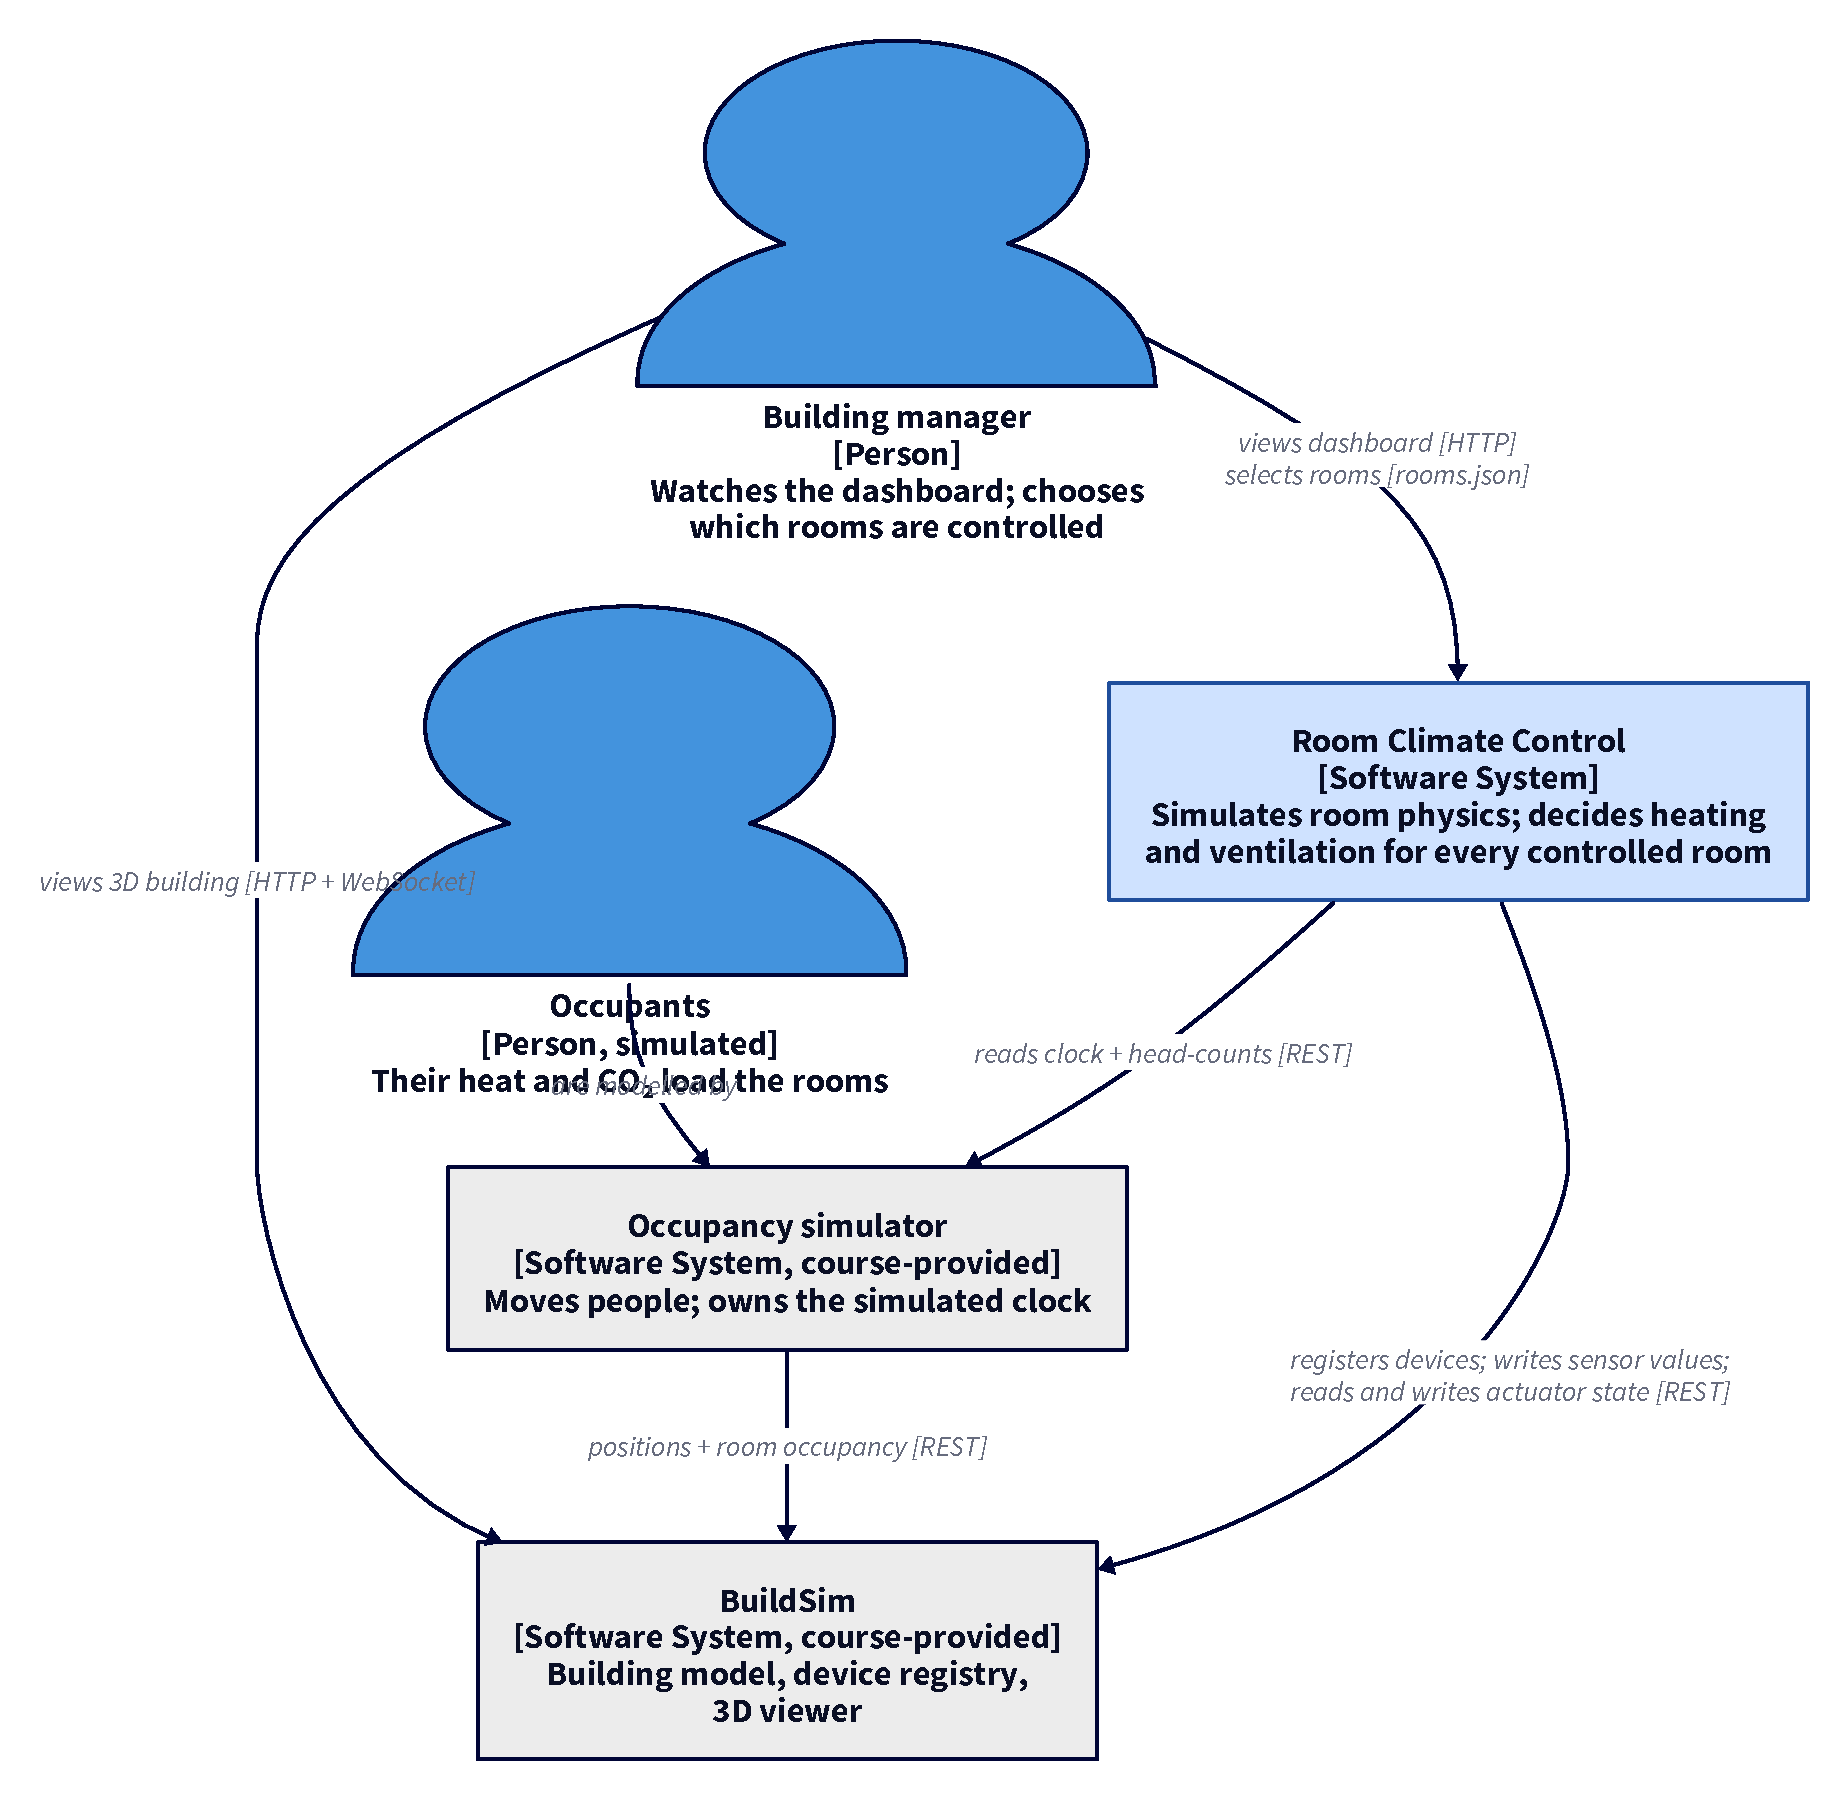
\includegraphics[width=0.78\textwidth]{figures/context.pdf}
\caption{C4 System Context. The system in scope is blue; course-provided systems
are grey. Every arrow is labelled with its purpose and protocol.}
\end{figure}

\subsection{4.2 Container diagram (C4 Level 2)}

Each box is one Docker service in \file{compose.yaml} or the generated
\file{services-compose.yaml}, and one Python file in the repository. The
\textbf{per-room device containers} are generated five times per controlled room:
an occupancy publisher, a temperature sensor, a CO₂ sensor, an HVAC actuator and
a ventilation actuator. The \textbf{shared services} run once: the physical
simulator, the decision maker, the MQTT broker, the metrics exporter, Prometheus
and Grafana. With five rooms that is 25 + 6 = 31 containers in our project plus
the two course systems.

The loop runs clockwise through the figure. The simulator waits for the
occupancy simulator's clock to advance five minutes, reads every room's actuator
state from BuildSim, steps the physics and publishes each room's physical values
to the broker. Each sensor writes its value into BuildSim and forwards it to the
decision maker. The decision maker publishes a command per loop; the actuators
apply it to BuildSim and acknowledge the value they read back. The next simulator
step reads that new actuator state.

\afterpage{%
\begin{landscape}
\begin{figure}[p]
\centering
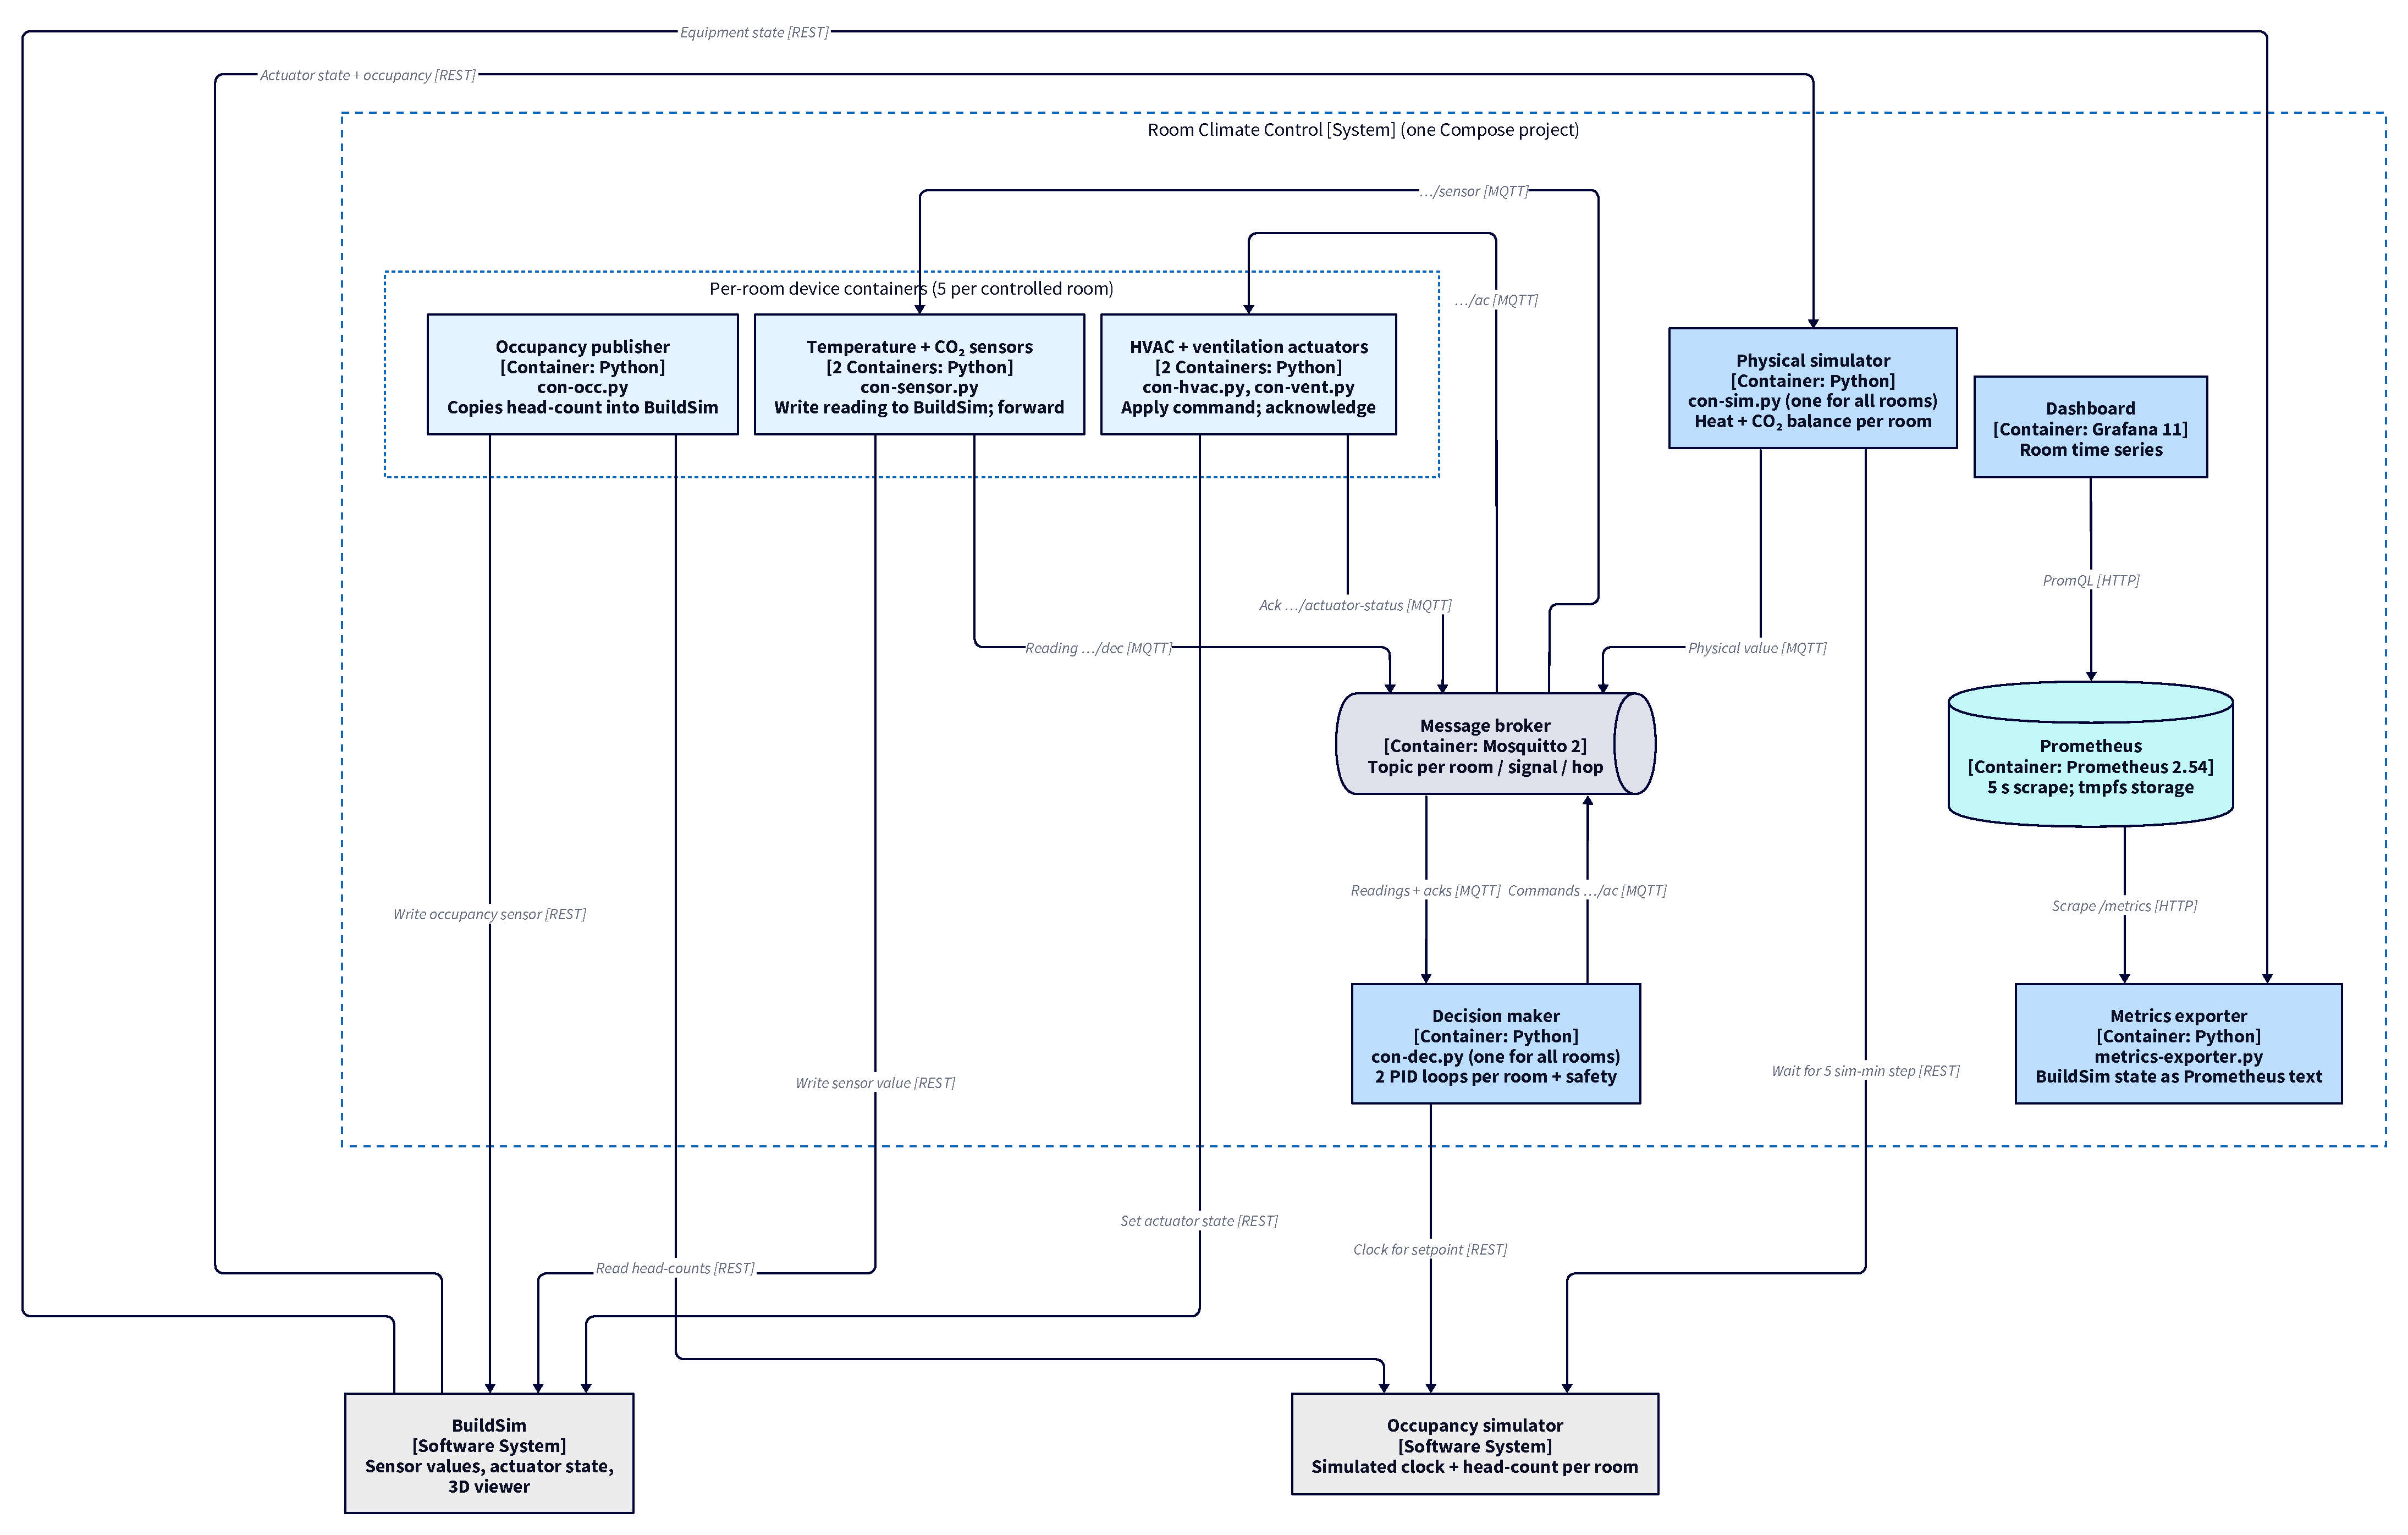
\includegraphics[width=\linewidth,height=0.86\textheight,keepaspectratio]{figures/container.pdf}
\caption{C4 Container diagram. The dashed boundary is the system (one Compose
project); the inner dotted group is instantiated once per controlled room.
External systems are grey.}
\label{fig:container}
\end{figure}
\end{landscape}}

\textbf{Why this split.} Each container has one job, and the ``reason for
separation'' column is the part we had to learn the hard way.

\begin{longtable}[]{@{}
  >{\raggedright\arraybackslash}p{(\columnwidth - 6\tabcolsep) * \real{0.20}}
  >{\raggedright\arraybackslash}p{(\columnwidth - 6\tabcolsep) * \real{0.30}}
  >{\raggedright\arraybackslash}p{(\columnwidth - 6\tabcolsep) * \real{0.10}}
  >{\raggedright\arraybackslash}p{(\columnwidth - 6\tabcolsep) * \real{0.40}}@{}}
\toprule
\textbf{Container} & \textbf{Responsibility (one job)} & \textbf{Count} & \textbf{Reason for separation} \\
\midrule
\endhead
\file{occ-*} (\file{con-occ.py}) & Copy one room's head-count into BuildSim & per room & Emulates a door counter; can fail alone \\
\file{sensor-*}, \file{sensor-co2-*} (\file{con-sensor.py}) & Own one BuildSim sensor; forward readings & 2 per room & A real sensor fails independently; fault tests stop exactly one \\
\file{hvac-*}, \file{vent-*} (\file{con-hvac.py}, \file{con-vent.py}) & Apply commands to one BuildSim actuator; acknowledge & 2 per room & Separate failure domains; the ack proves the value was applied \\
\file{sim} (\file{con-sim.py}) & Room physics for every room & 1 & The environment, not a device: one clock and one step for all rooms \\
\file{dec} (\file{con-dec.py}) & Two PID loops per room, fault detection & 1 & Decision logic evolves independently of devices; one process holds all controller state \\
\file{mosquitto} & Route readings, commands, acks & 1 & Decouples devices from the decision maker \\
\file{metrics-exporter} & Expose BuildSim state as Prometheus metrics & 1 & Monitoring must not load the control path \\
\file{prometheus}, \file{grafana} & Store recent metrics; dashboard & 1 each & Off-the-shelf; replaceable without touching control \\
\bottomrule
\end{longtable}

\subsection{4.3 Component diagram (C4 Level 3)}

The decision maker is the one container with internal structure worth drawing,
because since the consolidation it serves every room. At start-up the
\textbf{controller registry} reads \file{rooms.json} and builds two independent
controllers per simulated room. The \textbf{topic router} subscribes to each
controller's reading and acknowledgement topics (20 subscriptions for five rooms)
and hands every message to exactly one controller, so rooms share a process but
no state. Inside a controller, the \textbf{sensor health monitor} decides whether
a reading can be trusted; trusted readings go to the \textbf{PID regulator} with
the setpoint from the \textbf{setpoint scheduler}, distrusted ones trigger the
fail-safe output. The \textbf{command publisher} numbers every command, and the
\textbf{actuator ack monitor} expects that number back. A \textbf{health watchdog}
thread checks every controller once a real second, so a sensor that goes silent
is caught even though no message arrives to trigger the check.

\begin{figure}[H]
\centering
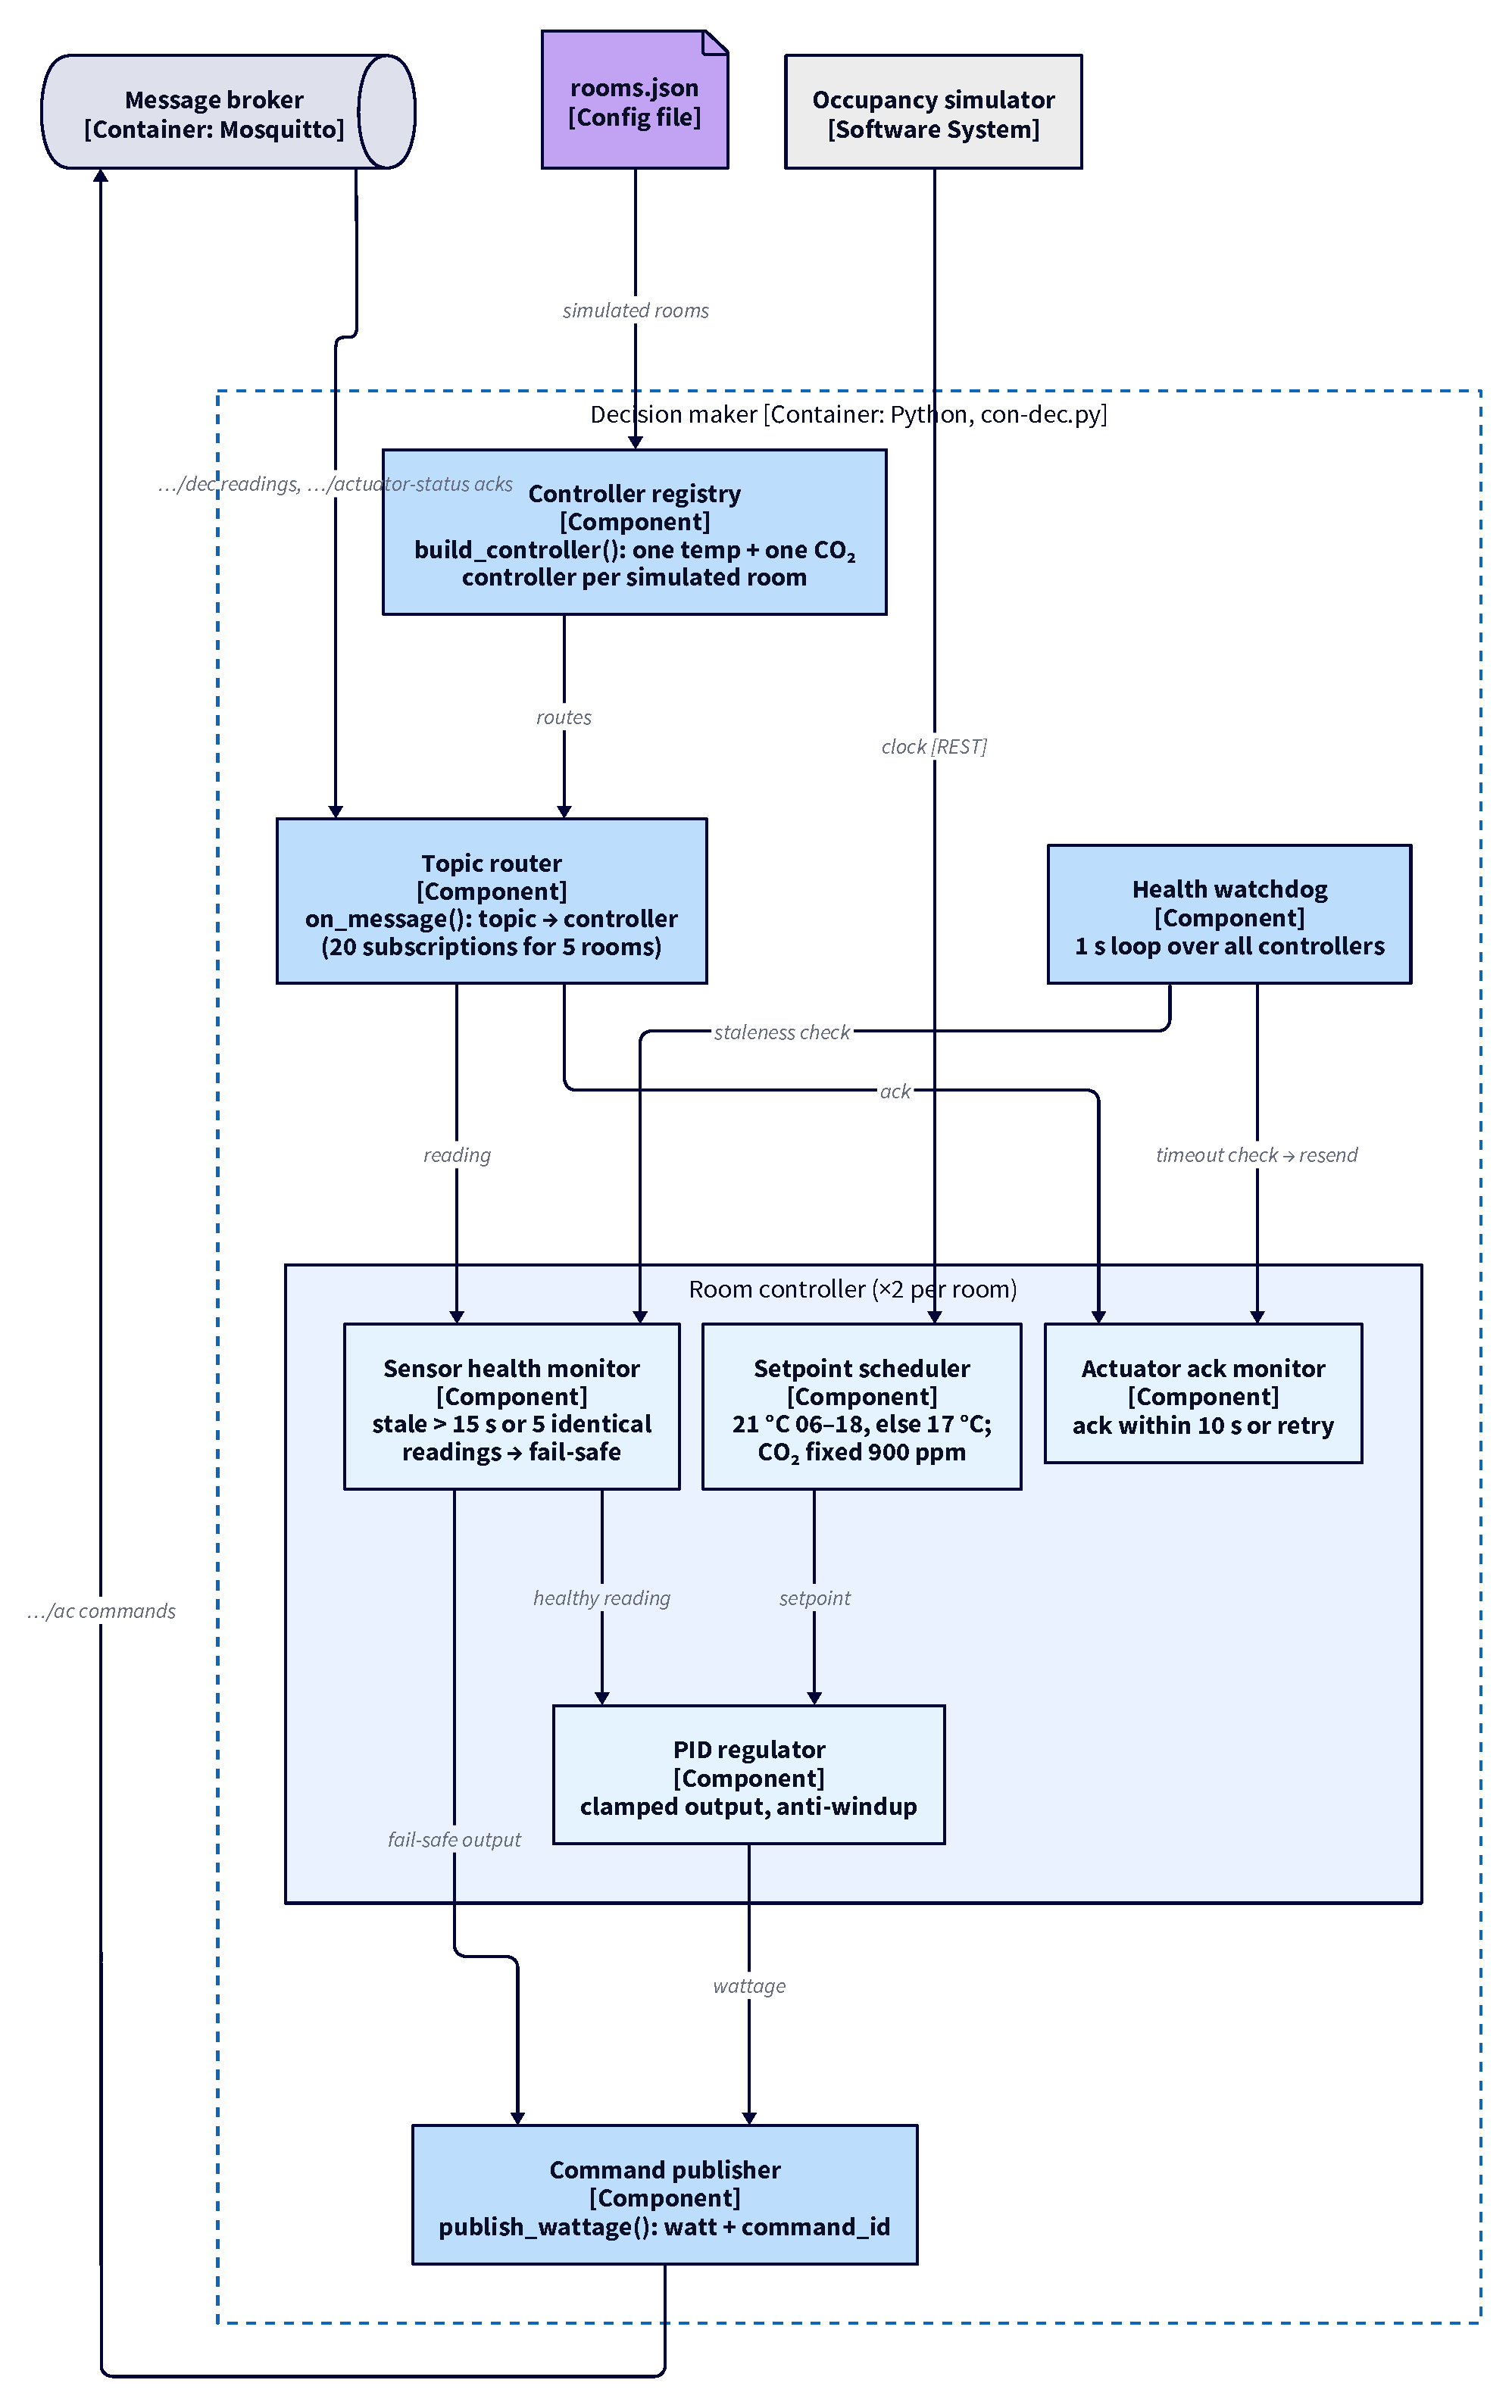
\includegraphics[height=0.78\textheight]{figures/component.pdf}
\caption{C4 Component diagram of the decision maker. The inner box is
instantiated twice per room (temperature and CO₂).}
\end{figure}

\needspace{14\baselineskip}
\subsection{4.4 Design decisions and alternatives}

\begin{longtable}[]{@{}
  >{\raggedright\arraybackslash}p{(\columnwidth - 8\tabcolsep) * \real{0.05}}
  >{\raggedright\arraybackslash}p{(\columnwidth - 8\tabcolsep) * \real{0.17}}
  >{\raggedright\arraybackslash}p{(\columnwidth - 8\tabcolsep) * \real{0.20}}
  >{\raggedright\arraybackslash}p{(\columnwidth - 8\tabcolsep) * \real{0.36}}
  >{\raggedright\arraybackslash}p{(\columnwidth - 8\tabcolsep) * \real{0.22}}@{}}
\toprule
& \textbf{Decision} & \textbf{Alternatives considered} & \textbf{Why this one (requirement)} & \textbf{Trade-off accepted} \\
\midrule
\endhead
D1 & One container per role, MQTT between them & Monolith with a shared SQLite file &
  Device faults can be injected and recovered one at a time (NFR-2, NFR-4); roles
  restart independently (NFR-5) & More processes and a broker to run \\
D2 & One decision maker for all rooms & One per room and signal (2 per room); one per room &
  952 containers for 119 rooms never started and would need about 23 GB (NFR-6,
  Section 11.5); routing by topic keeps rooms isolated in one process (NFR-4) & One process is a single point of failure for
  control; mitigated by restart and fail-safe (NFR-5) \\
D3 & One physical simulator for all rooms & One simulator per room &
  The physics is the environment, not a device: one clock read and one step per
  timestep; a failing room is skipped, not fatal (NFR-4) & A simulator crash stops
  physics for all rooms until restart \\
D4 & Keep sensors and actuators per room & Merge them into one device container &
  They are what fails in a real building, and per-device fault tests need them
  separate (NFR-2, NFR-3) & Memory grows by five containers per room (Section 11.5) \\
D5 & MQTT pub/sub for readings, commands and acks; topic per room, signal and hop &
  REST calls between services; one topic per room with a type field &
  Producers do not need to know consumers; the router maps a topic straight to a
  controller (NFR-1) & QoS 0, no persistence: a message sent during a broker outage
  is lost (Section 11.4) \\
D6 & Sensor process writes BuildSim; simulator hands values to it over MQTT &
  Simulator writes BuildSim and sensors poll it (course reference flow) &
  Each BuildSim sensor has exactly one writer, its device, and a dead sensor
  visibly stops updating BuildSim (NFR-2) & The ``physical'' link is modelled as
  a network message; one extra hop \\
D7 & Plant and controller separated & Ideal thermostat inside the simulator &
  Control can only be tested if the plant just applies actuator power (FR-1) &
  Must tune a controller instead of getting perfect control for free \\
D8 & Clamped PID with anti-windup & On/off with hysteresis; MPC or learned policy &
  Proportional power with no oscillation, three parameters, and a closed-loop
  unit test that reaches and holds the setpoint (FR-1, FR-3) & Gains are tuned
  against real seconds, so they depend on the clock factor (Section 13) \\
D9 & Fail-safe: heating 0 W, ventilation 600 W & Hold last command & A frozen
  value must not keep driving the actuator; fresh air beats energy when CO₂ is
  unknown (NFR-2) & Rooms cool during a sensor outage \\
D10 & Course occupancy simulator & Own timetable from \file{Lectures.json}; random
  density sampler & Realistic agent movement and lectures, same data as the 3D
  view (FR-4) & External dependency with a broken health check (Section 9) \\
D11 & Time-scheduled setback (21/17 °C) & Occupancy-based setback & Predictable and
  needs no occupancy forecast; lecture occupancy is bursty (FR-2) & Empty rooms are
  heated all day (Section 13) \\
D12 & Prometheus + Grafana, dashboard as code & Custom web UI or BuildSim
  session overlay; time-series DB & Provisioned with the stack, zero code for
  plots (Section 12) & No history across restarts; decisions not shown \\
D13 & Generate per-room services from \file{rooms.json} & Hand-written compose
  file & One flag per room (FR-5); the 400 KB generated file was unmaintainable by
  hand & Regenerate and rebuild after every change \\
\bottomrule
\end{longtable}

%% ===========================================================================
\section{5. Interfaces and data contracts}

Two patterns are used, each where it fits. \textbf{MQTT} (Mosquitto 2, port
1883, QoS 0, not retained) carries everything that flows between our own
services, because a reading has a producer and a consumer that should not know
each other, and because the decision maker can subscribe to every room on one
connection. \textbf{REST} (HTTP + JSON) is used for every call to BuildSim and
the occupancy simulator: each is a one-to-one request whose result the caller
needs, and both systems only offer REST. All payloads are JSON objects; numeric
values are sent as strings, matching BuildSim's \texttt{"data\_type":"text"} sensors.

\textbf{MQTT topics.} Every topic has the form
\topic{\{level\}/\{room\}/\{signal\}/\{hop\}}, where \topic{level} is the floor
number (\topic{0}), \topic{room} the URL-quoted BuildSim room name, \topic{signal}
is \topic{temp} or \topic{co2}, and \topic{hop} says where the message is in the
loop. One topic per hop makes each process's subscriptions explicit and lets the
decision maker map a topic to a controller with a dictionary lookup.

\begin{longtable}[]{@{}
  >{\raggedright\arraybackslash}p{(\columnwidth - 6\tabcolsep) * \real{0.31}}
  >{\raggedright\arraybackslash}p{(\columnwidth - 6\tabcolsep) * \real{0.17}}
  >{\raggedright\arraybackslash}p{(\columnwidth - 6\tabcolsep) * \real{0.34}}
  >{\raggedright\arraybackslash}p{(\columnwidth - 6\tabcolsep) * \real{0.18}}@{}}
\toprule
\textbf{Topic} & \textbf{From → to} & \textbf{Payload (example)} & \textbf{Rate} \\
\midrule
\endhead
\topic{0/A108/temp/sensor} & sim → temp sensor & \texttt{\{"value":"20.04"\}} (°C) & 1 per step \\
\topic{0/A108/co2/sensor} & sim → CO₂ sensor & \texttt{\{"value":"937.6"\}} (ppm) & 1 per step \\
\topic{0/A108/temp/dec} & sensor → dec & \texttt{\{"value":"20.04"\}} & 1 per step \\
\topic{0/A108/co2/dec} & sensor → dec & \texttt{\{"value":"937.6"\}} & 1 per step \\
\topic{0/A108/temp/ac} & dec → HVAC & \texttt{\{"watt":"6345.2",\allowbreak"command\_id":41\}} or \texttt{\{"set\_temp":"21"\}} & 1 per step; setpoint on change \\
\topic{0/A108/co2/ac} & dec → vent & \texttt{\{"watt":"188.0",\allowbreak"command\_id":41\}} (0–600) & 1 per step \\
\topic{0/A108/temp/actuator-status} & HVAC → dec & \texttt{\{"command\_id":41,\allowbreak"state":"6345.2"\}} & per command \\
\topic{0/A108/co2/actuator-status} & vent → dec & \texttt{\{"command\_id":41,\allowbreak"state":"188.0"\}} & per command \\
\bottomrule
\end{longtable}

\textbf{Command semantics.} \texttt{command\_id} increases by one per command
and per loop. An acknowledgement is accepted only if its \texttt{command\_id}
equals the latest command's and its \texttt{state} equals the commanded value
within 0.01; anything else counts as a failed apply. An unacknowledged command is
resent unchanged after 10 s real (Section 7.1). The \texttt{set\_temp} message is
informational: the HVAC actuator stores it in BuildSim for the viewer and the
dashboard, but the power command is what heats.

\textbf{BuildSim REST calls.} Device ids follow fixed patterns, so any process can
compute another's ids from the room name.

\begin{longtable}[]{@{}
  >{\raggedright\arraybackslash}p{(\columnwidth - 6\tabcolsep) * \real{0.18}}
  >{\raggedright\arraybackslash}p{(\columnwidth - 6\tabcolsep) * \real{0.36}}
  >{\raggedright\arraybackslash}p{(\columnwidth - 6\tabcolsep) * \real{0.30}}
  >{\raggedright\arraybackslash}p{(\columnwidth - 6\tabcolsep) * \real{0.16}}@{}}
\toprule
\textbf{Caller} & \textbf{Call} & \textbf{Body / result} & \textbf{When} \\
\midrule
\endhead
sensor, HVAC, vent, occ & \texttt{POST /api/equipment}, then \texttt{POST /api/equipment/\{eq\}/sensors} or \texttt{/actuators} &
  equipment \texttt{temp-A108}, \texttt{co2-A108}, \texttt{hvac-A108}, \texttt{vent-A108}, \texttt{occupancy-A108}; devices \texttt{A108-temp}, \texttt{A108-co2}, \texttt{A108-watt}, \texttt{A108-set}, \texttt{A108-vent}, \texttt{A108-occupancy} & start-up \\
sensor, occ & \texttt{PUT /api/sensors/\{id\}/value} & \texttt{\{"data\_type":"text",\allowbreak"value":"20.04"\}} & each reading \\
HVAC, vent & \texttt{PUT /api/actuators/\{id\}/state}, then \texttt{GET /api/actuators/\{id\}} & \texttt{\{"state":"6345.2"\}}; the GET's \texttt{state} is acknowledged & each command \\
sim & \texttt{GET /api/actuators/A108-watt}, \texttt{…/A108-vent}, \texttt{GET /api/sensors/A108-occupancy} & \texttt{state}, \texttt{value} as strings & each step, per room \\
sim & \texttt{GET /api/building/floors/level0} & room \texttt{area} & start-up \\
exporter & \texttt{GET /api/equipment} & every device with its current value & each scrape (5 s) \\
\bottomrule
\end{longtable}

\textbf{Occupancy simulator.} \texttt{GET /api/state} returns, among other
things, the clock and a list of rooms; the simulator and occupancy publishers use
these two fields:

\begin{lstlisting}
{"sim": {"clock": {"time": "2026-10-12T08:24:53Z", "time_of_day": "08:24",
                   "weekday": "Monday", "factor": 60, "running": true},
         "rooms": [{"name": "A108", "level": "level0", "role": "lecture",
                    "area_m2": 122.875, "capacity": 61, "occupants": 29}]}}
\end{lstlisting}

\textbf{Monitoring.} \texttt{GET /metrics} on the exporter returns Prometheus
text with eight gauges: \texttt{room\_temperature\_celsius},
\texttt{room\_co2\_ppm}, \texttt{room\_occupancy\_people},
\texttt{room\_power\_consumption\_watts}, \texttt{room\_ventilation\_command\_watts}
and \texttt{room\_set\_temperature\_celsius}, labelled \texttt{room}, plus
\texttt{building\_outside\_temperature\_celsius} and
\texttt{building\_occupancy\_sim\_time\_seconds}.

%% ===========================================================================
\section{6. Simulating the sensor values (the physical model)}

BuildSim has rooms but no physics, so the simulator (\file{con-sim.py}) produces
every temperature and CO₂ value. It is deliberately simple, but it has the three
properties the controller needs: slow thermal dynamics, a CO₂ response to people,
and a genuine response to both actuators.

\textbf{Time.} The simulator polls the occupancy simulator's clock every 0.5 s
real and steps when five simulated minutes have passed ($\Delta t = 300$ s).
Outside temperature is interpolated linearly from \file{Weather.json}, which has
one value every three hours for Monday to Friday.

\textbf{Occupancy.} The head-count $n$ of each room comes from the occupancy
simulator via the room's occupancy sensor in BuildSim. The occupancy simulator is
agent-based: each person gets a timetable for the day (arrival 08:00–10:00,
optional fika breaks, lunch 12:00–13:00 in or out of the building, departure
16:00–19:00); students attend one to three lectures in five slots between 08:15
and 18:00, and lectures are packed into the fewest rooms that seat the demand.
People walk between rooms along BuildSim's walkable graph at 1.3 m/s. All five of
our rooms classify as lecture rooms (61–94 seats), so their occupancy jumps from
0 to 20–60 at slot boundaries, a hard test for the CO₂ loop.

\textbf{Temperature.} Each room is two thermal nodes: the air (temperature $T$,
capacity $C_a = \rho c_p V$) and the room's thermal mass (temperature $T_m$,
capacity $C_m = c_m A$):
\begin{align}
C_a \frac{dT}{dt} &= P_\text{hvac} + q_\text{occ}\, n
  - (U A_w + \rho c_p V \tfrac{\text{ACH}_0}{3600})(T - T_\text{out})
  + h A (T_m - T), \\
C_m \frac{dT_m}{dt} &= -h A (T_m - T),
\end{align}
with floor area $A$, volume $V = 3A$, exterior wall area $A_w = 3\,L_w$ from the
wall length $L_w$ in \file{rooms.json}, $U = 0.25$ W/m²K, background air change
$\text{ACH}_0 = 0.5$ h$^{-1}$, $c_m = 165$ kJ/m²K, air--mass coupling $h = 8$ W/m²K,
and $q_\text{occ} = 75$ W sensible heat per person. $P_\text{hvac}$ is the HVAC
actuator's power as read from BuildSim. The equations are integrated with
explicit Euler in sub-steps of at most 60 s (six 50 s sub-steps per step), which
keeps the air node stable.

\textbf{CO₂.} With ventilation power $P_v$ mapped linearly to $0$–$3$ air changes
per hour, $\lambda = 3\min(P_v/600, 1)/3600$ s$^{-1}$, and generation
$g = n\, G / V \cdot 10^6$ ppm/s with $G = 5$ mL/s per person, the well-mixed mass
balance has the exact solution over a step
\begin{equation}
C(t+\Delta t) = C_\text{eq} + \big(C(t) - C_\text{eq}\big)e^{-\lambda \Delta t},
\qquad C_\text{eq} = 420 + g/\lambda,
\end{equation}
and $C(t+\Delta t) = C(t) + g\,\Delta t$ when $\lambda = 0$. Using the exact
solution rather than an Euler step means a 5-minute step cannot overshoot below
the outdoor 420 ppm.

\textbf{Sensor noise.} Each published value gets Gaussian noise
(σ = 0.2 °C, σ = 10 ppm, CO₂ clamped at 420 ppm). The noise is not cosmetic: it
is what lets the stuck-sensor rule (five identical readings) work, because a live
sensor never repeats a value exactly.

\textbf{Closing the loop.} Both actuators enter the equations: $P_\text{hvac}$
directly as heat, $P_v$ through $\lambda$. A command applied in step $k$ is read
at the start of step $k+1$, so actuation lags one step (5 min), the same as a
real BMS polling cycle.

\begin{figure}[H]
\centering
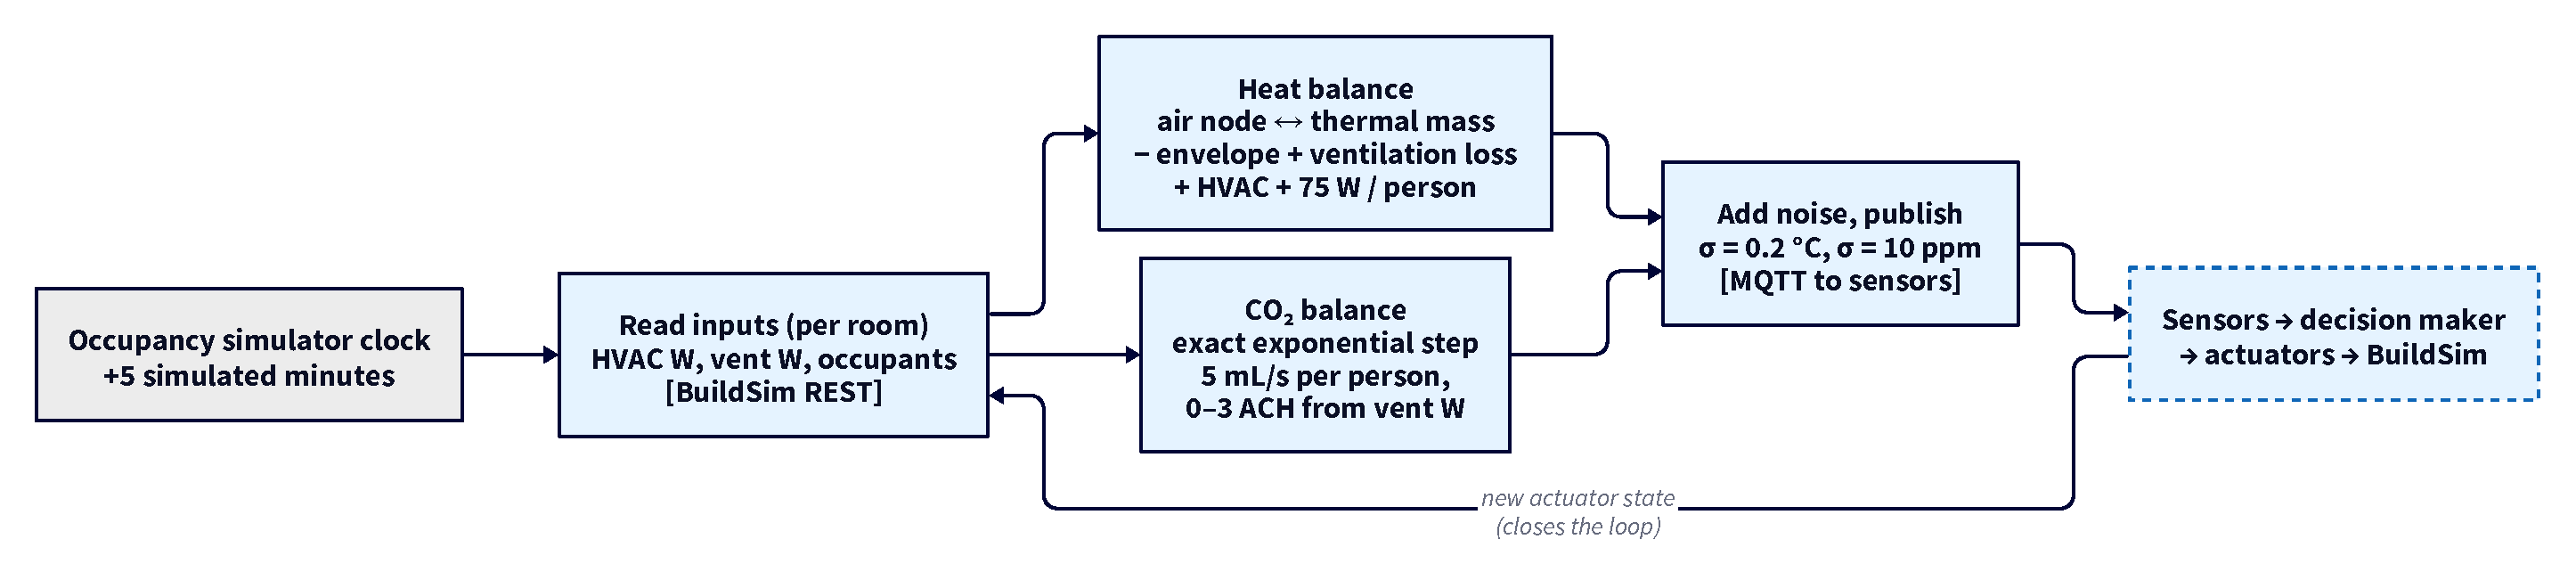
\includegraphics[width=\textwidth]{figures/simloop.pdf}
\caption{One simulator step. The dashed path is the rest of the system; its
effect re-enters as actuator state at the next step.}
\end{figure}

%% ===========================================================================
\section{7. Autonomous services and data pipeline}

\subsection{7.1 The autonomous service}

The decision maker (\file{con-dec.py}) runs two control loops per room: heating
power from temperature, and ventilation power from CO₂.

\textbf{Algorithm.} Each loop is a PID regulator acting on every incoming reading:
\[
u = \operatorname{clamp}_{[0,\,u_\text{max}]}\!\Big(K_p e + K_i \!\int\! e\,dt - K_d \tfrac{dy}{dt}\Big),
\]
with $e = T_\text{sp} - T$ for heating and $e = C - C_\text{sp}$ for ventilation.
The derivative acts on the measurement, not the error, so a setpoint change does
not kick the output. The integral is only updated when the unclamped output is
inside $[0, u_\text{max}]$ or the error would move it back inside (conditional
integration), which prevents wind-up during the hours-long warm-up.

\begin{longtable}[]{@{}lllllll@{}}
\toprule
\textbf{Loop} & \textbf{Setpoint} & $K_p$ & $K_i$ & $K_d$ & $u_\text{max}$ & \textbf{Fail-safe} \\
\midrule
\endhead
Heating & 21 °C (06–18), 17 °C & 1000 W/°C & 10 W/(°C·s) & 0 & 30 kW & 0 W \\
Ventilation & 900 ppm & 5 W/ppm & 0.001 W/(ppm·s) & 0 & 600 W & 600 W \\
\bottomrule
\end{longtable}

\textbf{Why PID.} The requirement is to hold a setpoint on a slow, first-order-ish
plant with a known actuator range. A PID does that with three interpretable
parameters, its behaviour can be verified in a closed-loop unit test against the
same physics code (T-1, T-2), and its output is proportional, so it does not
cycle the HVAC on and off the way a hysteresis thermostat would. A learned
or optimising controller would need a model or data we do not have, and would be
harder to verify for a safety-relevant function. The setpoint schedule is a simple
clock rule for the same reason (D11).

\textbf{Inputs, outputs, integration.} Inputs are the readings on
\topic{…/dec} and the clock from the occupancy simulator (for the setpoint).
Outputs are the numbered commands on \topic{…/ac}. All controllers share one MQTT
connection; the router delivers each message to one controller, and malformed
payloads or an unreachable occupancy simulator are caught and logged per message
without touching the other controllers. An unexpected exception type, however,
would propagate into the shared MQTT network thread and stop delivery to every
room; the handlers catch only the errors we have seen.

\textbf{Failure and safety behaviour.}
\begin{itemize}
\tightlist
\item \textbf{Stale or stuck input.} The sensor health monitor flags a loop if no
  reading arrived for 15 s real (three missed steps) or the last five readings
  were identical. The loop then publishes its fail-safe output once and ignores
  readings until a fresh, changed one arrives. The 1 s watchdog thread makes the
  stale check independent of message arrival.
\item \textbf{Actuator does not apply.} Every command carries an id; if no
  matching acknowledgement arrives within 10 s real, the watchdog resends the last
  command and restarts the timer, until it is confirmed.
\item \textbf{Decision maker unavailable.} Actuators hold their last value. Docker
  restarts a crashed process (\texttt{restart: unless-stopped}); controllers start
  empty and resume from the next reading. Section 11.4 shows the gap in this: a
  container stopped with \texttt{docker kill} is not restarted.
\end{itemize}

\subsection{7.2 The data pipeline}

The control path keeps no history on purpose: each controller holds only its last
reading, its integral and its pending command, and the readings themselves arrive
over MQTT. Storing and querying readings on the control path would add latency
and a failure mode for no control benefit, since the PID only needs the current
value.

For monitoring, a separate pipeline samples BuildSim, which already holds the
latest value of every sensor and actuator. On each Prometheus scrape (every 5 s
real, i.e.\ every simulated 5 minutes) the metrics exporter reads the whole
equipment registry and the occupancy clock and returns eight gauges labelled by
room. Prometheus stores them in a tmpfs volume, so history lasts only as long as the
container: this is a deliberate choice for a laptop demo (nothing to clean up, no
disk growth) and a real limitation for long-term analysis (Section 13).

\textbf{Data quality.} Missing and stale readings are handled where they matter,
in the decision maker (above). The exporter skips values it cannot parse and logs
them, and returns HTTP 503 when BuildSim or the occupancy simulator is unreachable,
so Prometheus records a gap instead of a wrong number. Duplicates cannot arise
because the exporter reads current state, not a stream.

\begin{figure}[H]
\centering
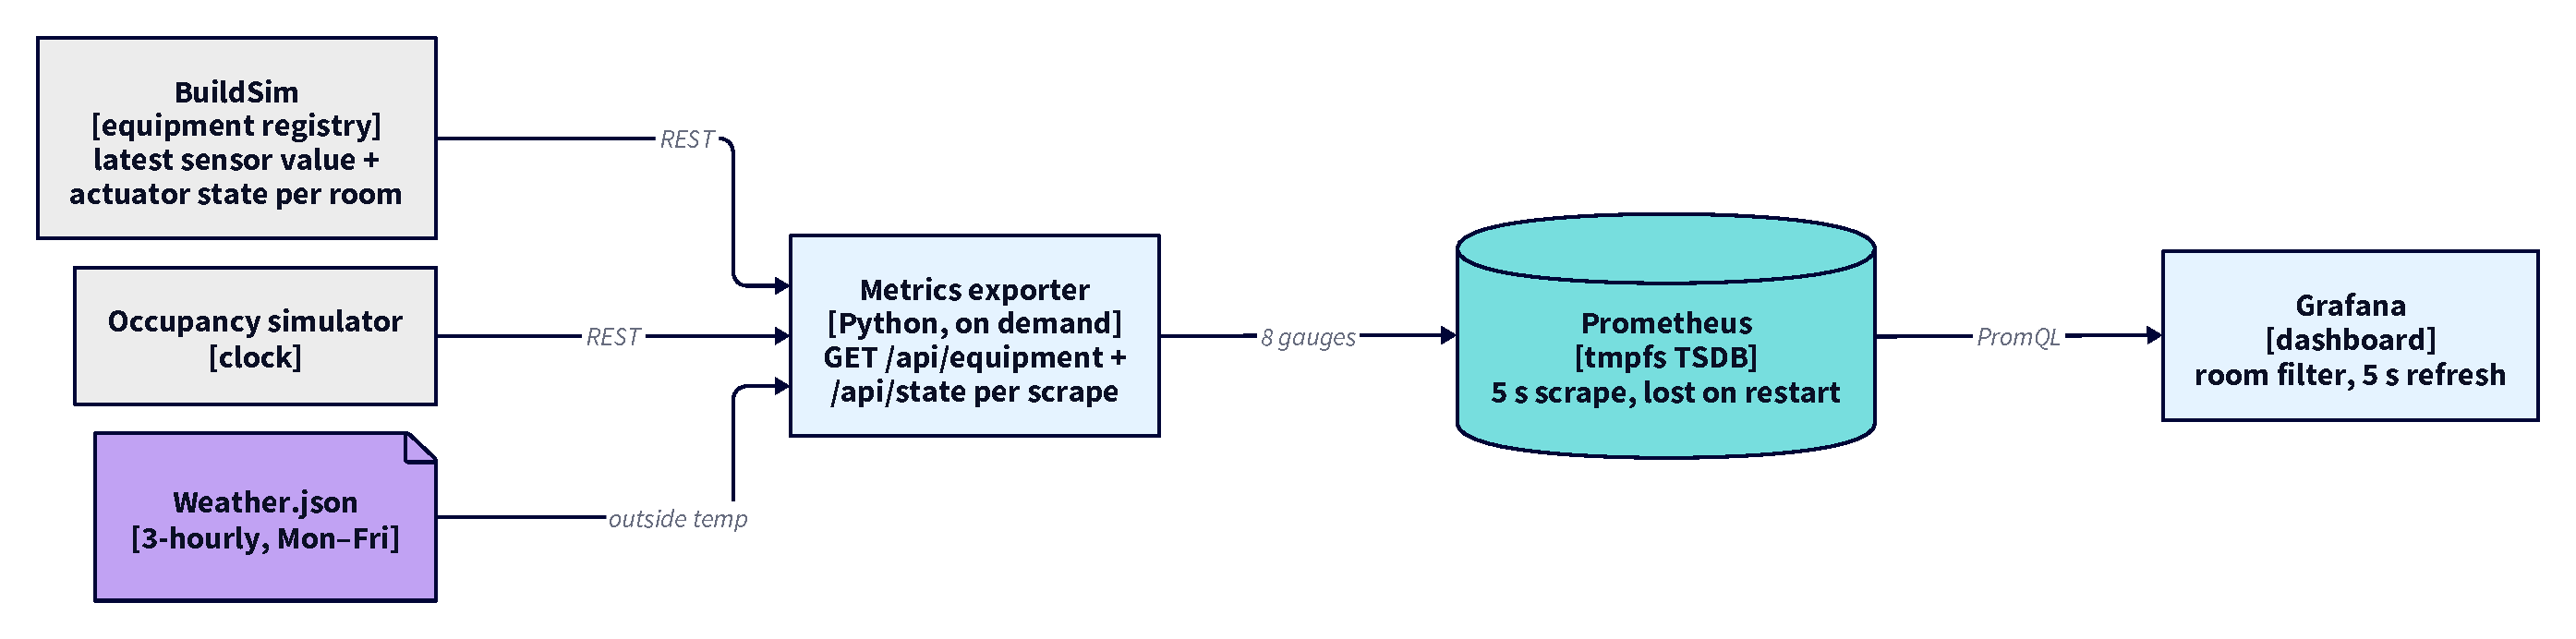
\includegraphics[width=\textwidth]{figures/pipeline.pdf}
\caption{Monitoring pipeline. Control does not read from it (dashed arrow).}
\end{figure}

%% ===========================================================================
\section{8. Behaviour}

\subsection{8.1 Key scenario (dynamic diagram)}

The scenario is the start of a lecture, taken from the logs of the measured run
(Section 11) with real timestamps and values. At 08:09 on Monday 29 students
arrived in A108; CO₂ crossed 900 ppm at 08:14 and the decision maker answered
with 32 W of ventilation. Figure~\ref{fig:dynamic} follows the next step. The
simulator steps when the clock reaches 08:19:47 (1), reads A108's actuators and
head-count from BuildSim (2), and computes 956.6 ppm including sensor noise (3).
The CO₂ sensor writes the value into BuildSim, where the 3D viewer shows it, and
forwards it (4–7). The router hands it to A108's CO₂ controller, whose PID turns
56.6 ppm of excess into 283.32 W (8–9). The ventilation actuator applies it,
reads it back and acknowledges command 7 (10–14): 50 ms after the decision and
93 ms after the simulator published, measured on the container clock. The step
at 08:24:53 reads the new
power (15): 1.4 air changes per hour pull CO₂ back to 911.6 ppm.

Two timing facts are visible here that static diagrams hide. The actuation lags
one step, because the simulator reads actuator state at the start of a step;
and the whole message chain takes about a tenth of a second, so the 5 s step,
not the network, sets the control rate.

\afterpage{%
\begin{landscape}
\begin{figure}[p]
\centering
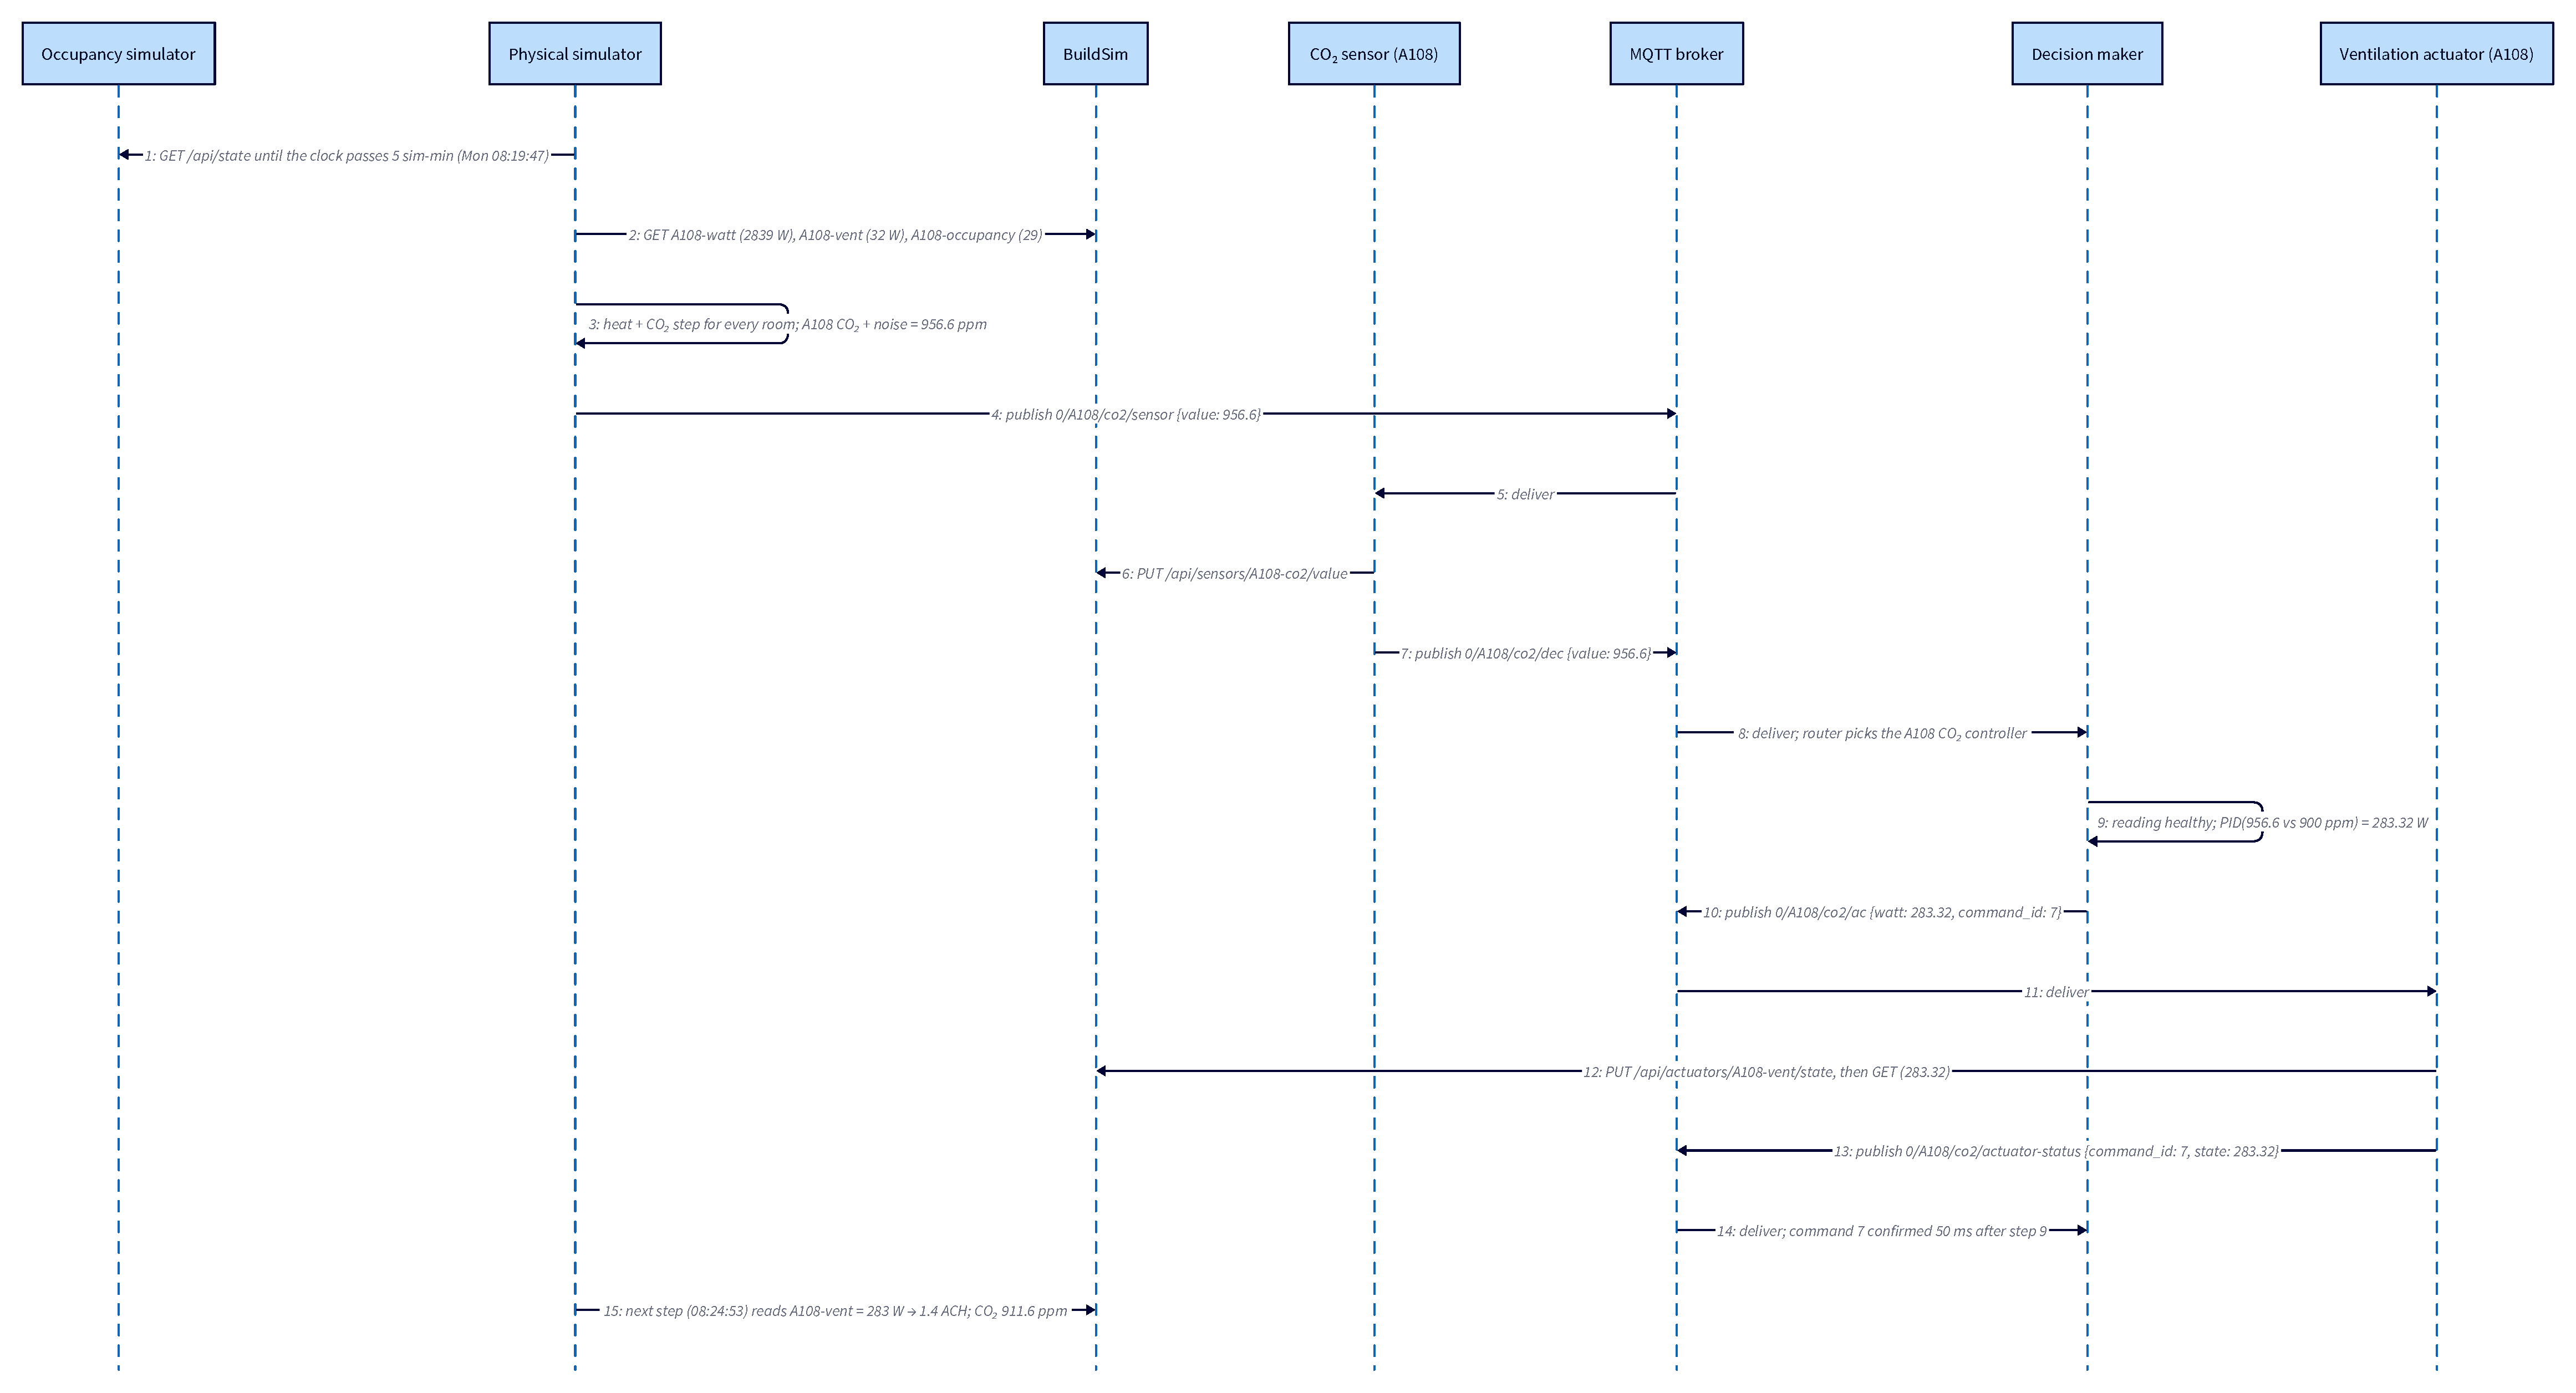
\includegraphics[width=\linewidth,height=0.86\textheight,keepaspectratio]{figures/dynamic.pdf}
\caption{C4 Dynamic diagram: one simulation step for the CO₂ loop of room A108
during a lecture.}
\label{fig:dynamic}
\end{figure}
\end{landscape}}

\subsection{8.2 Process lifecycle (state diagram)}

Each of the decision maker's controllers (two per room) has the lifecycle below;
every transition is a branch in \file{con-dec.py} or \file{control\_safety.py}. A
controller starts in \emph{Waiting} and has 15 s real to receive its first reading
before it fails safe, so a room whose sensor never starts is not left uncontrolled.
\emph{Controlling} and \emph{Fail-safe} describe the sensor side; \emph{Awaiting
ack} and \emph{Retrying} describe the actuator side and run alongside them. The
fault-injection runs in Section 11.4 drive a controller through every transition.

\begin{figure}[H]
\centering
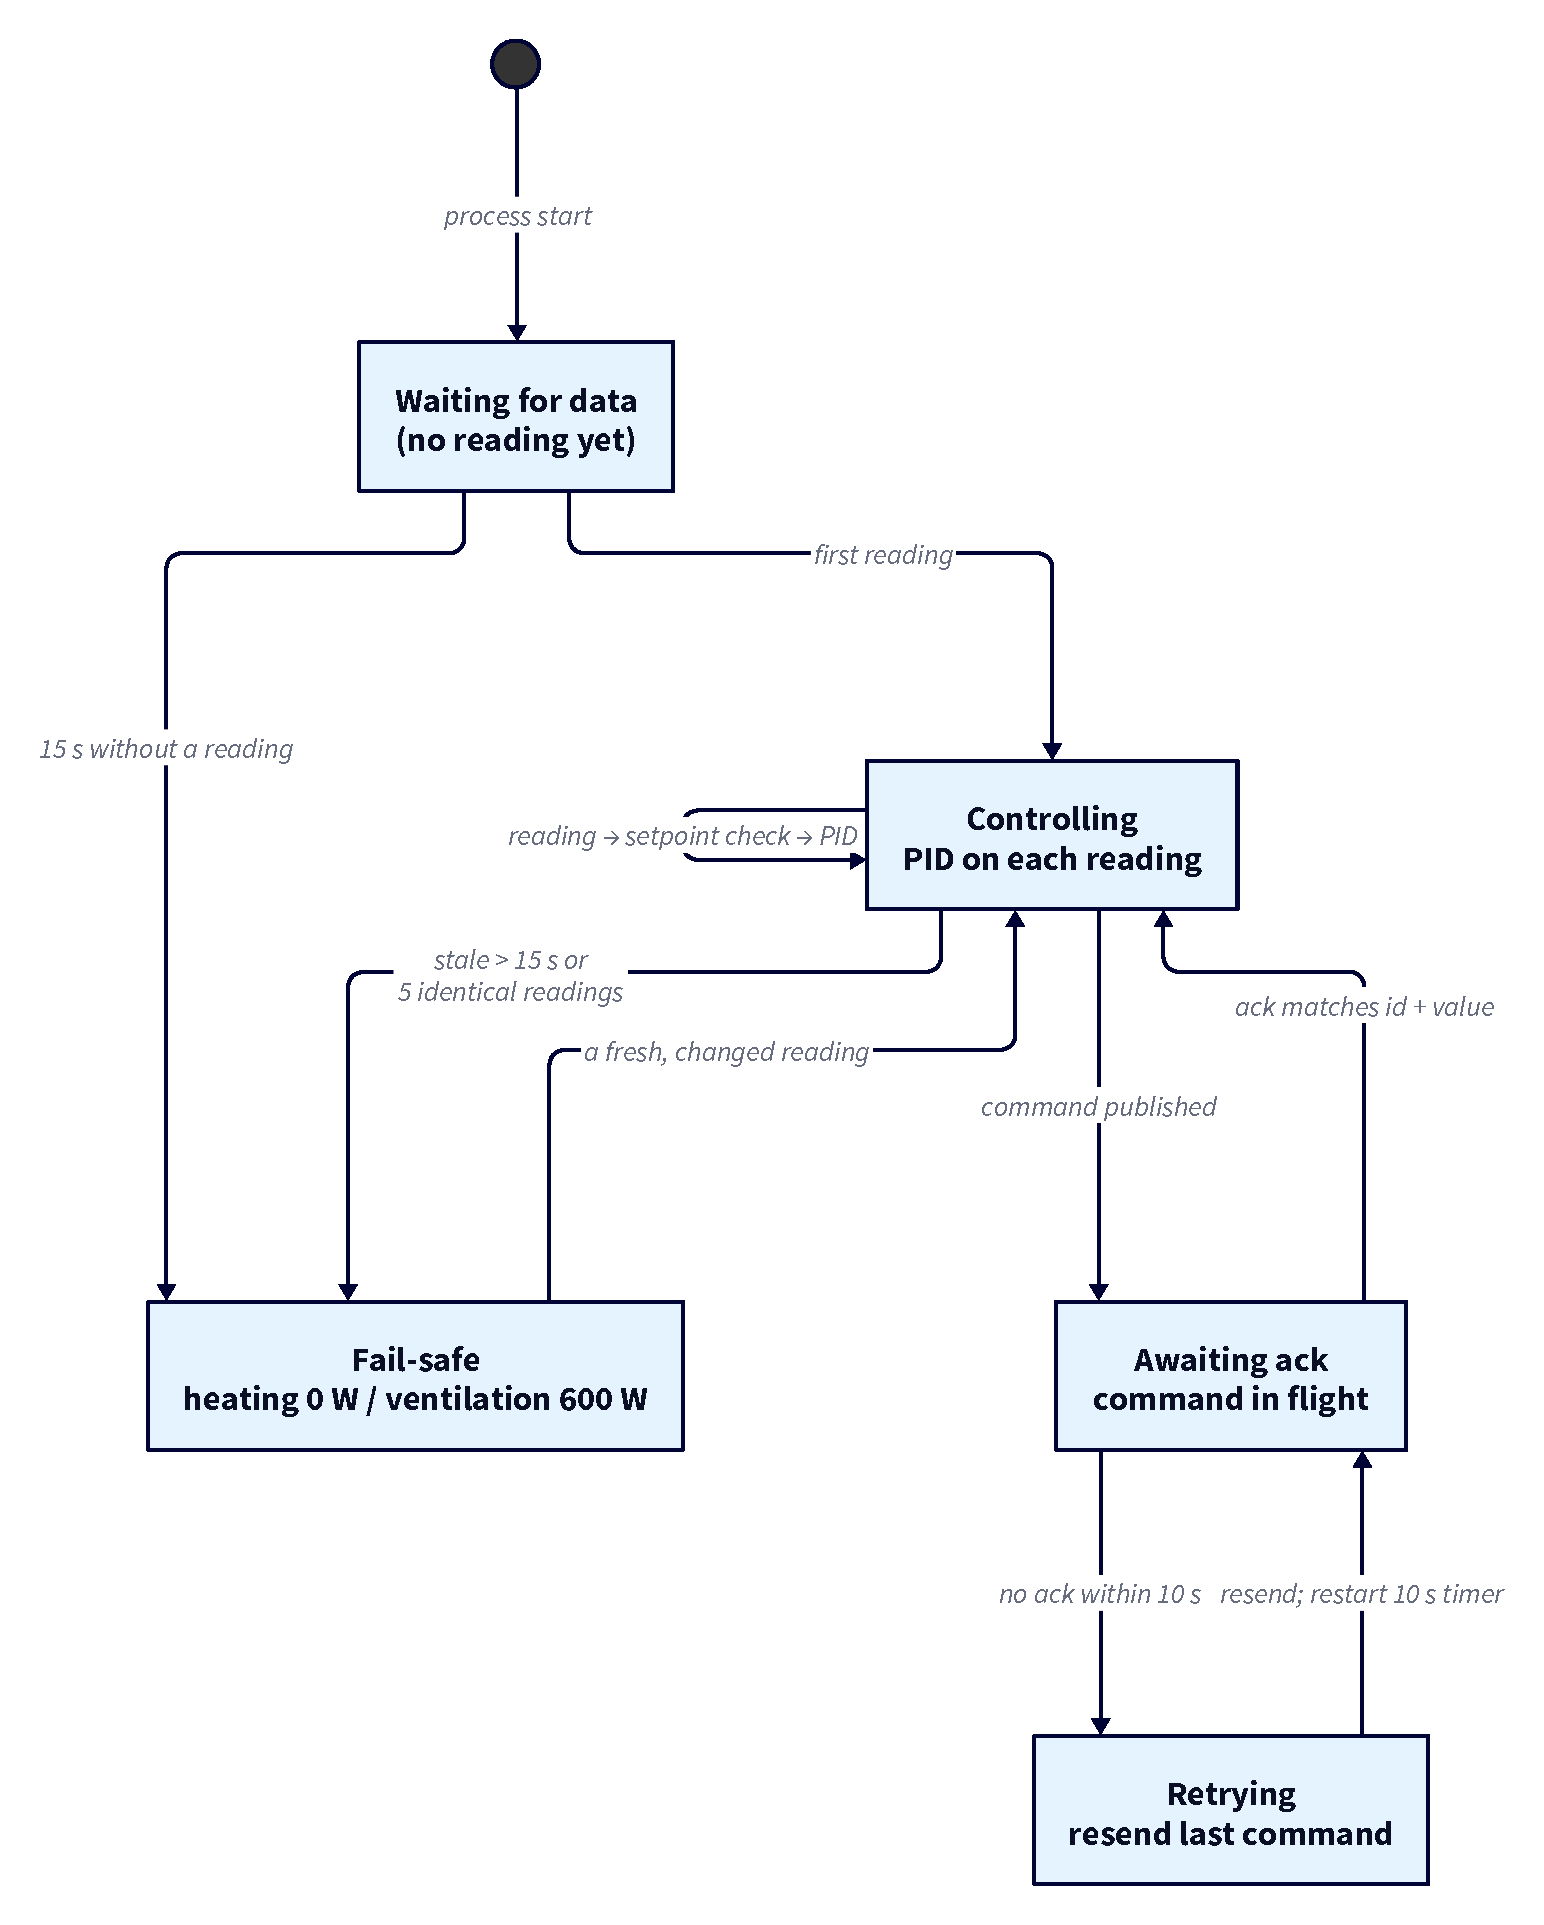
\includegraphics[width=0.62\textwidth]{figures/state.pdf}
\caption{Lifecycle of one controller in the decision maker.}
\end{figure}

%% ===========================================================================
\section{9. Deployment and component view}

Everything runs on one laptop: Docker Desktop's Linux VM (8 GB, 12 vCPU on the
measurement machine) hosts one Compose project on a private bridge network, where
services find each other by name (\texttt{buildsim:9090},
\texttt{mosquitto:1883}). Only the browser-facing ports are published, and only
on 127.0.0.1: Grafana 3000, Prometheus 9091, BuildSim 9090, occupancy UI 8081,
MQTT 1883. All our services are built from one image (\texttt{d7065e-python},
Python 3.12-slim with \texttt{requests} and \texttt{paho-mqtt}); each container
runs a different script with different arguments.

\begin{figure}[H]
\centering
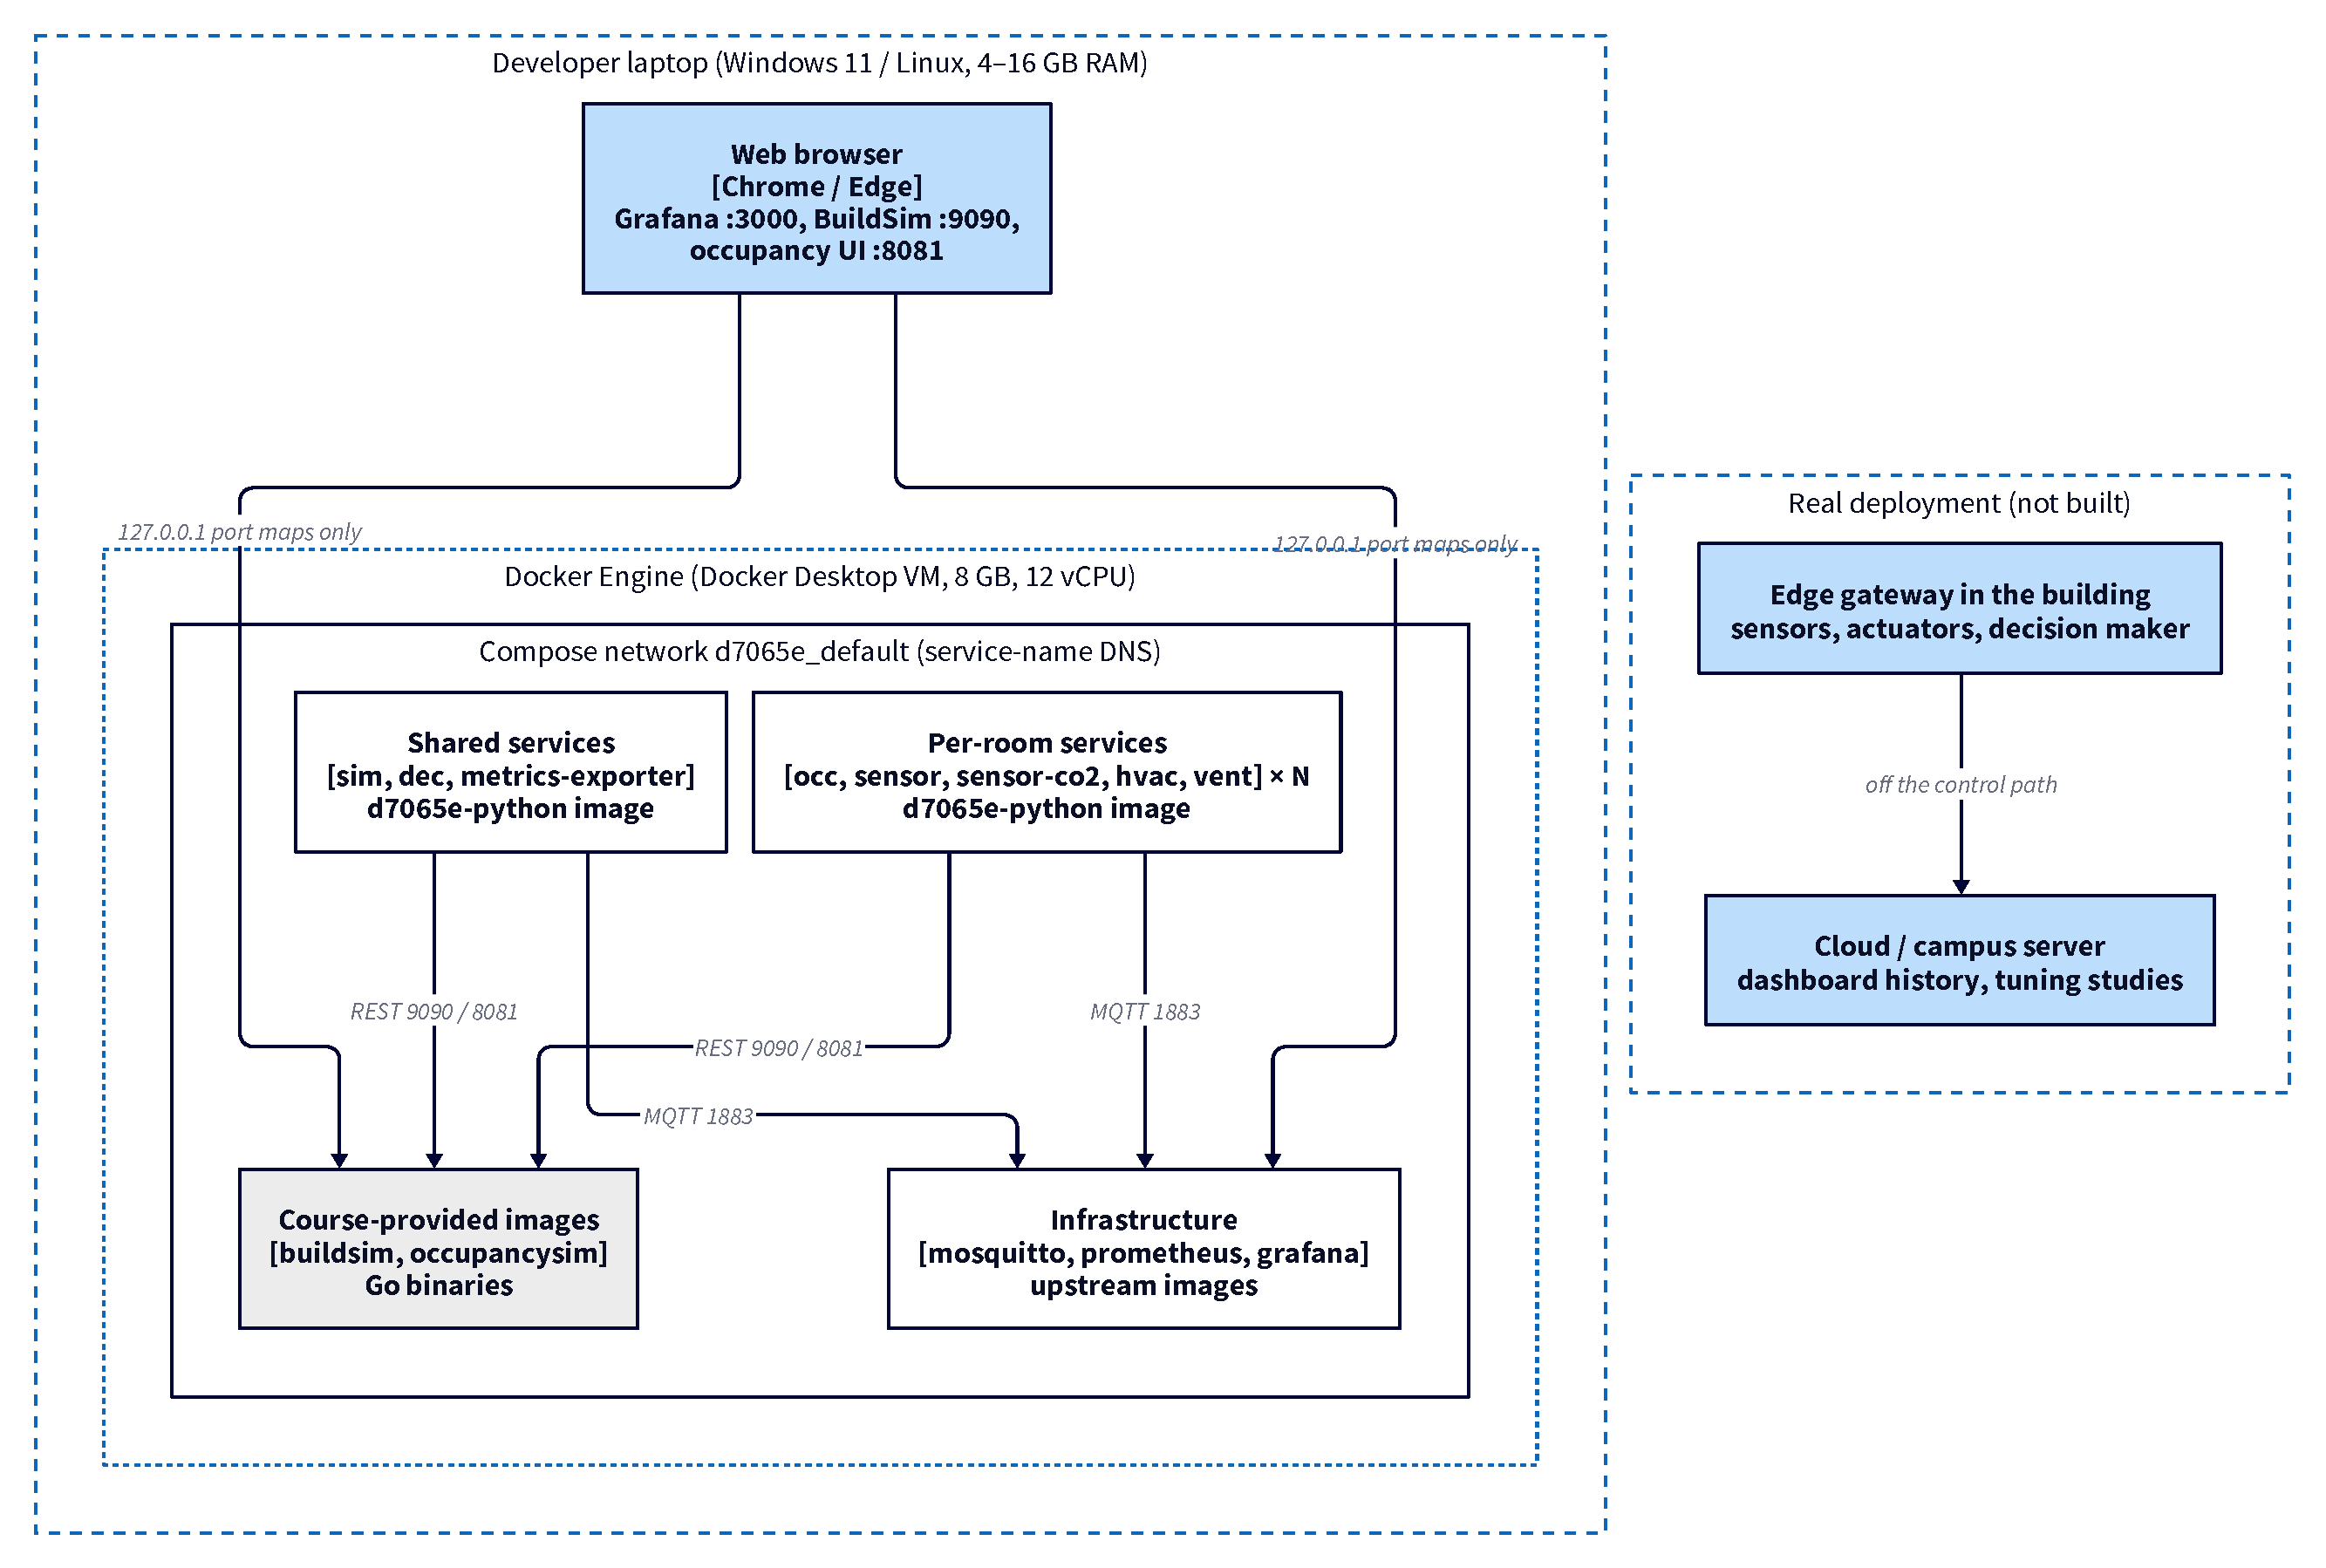
\includegraphics[width=\textwidth]{figures/deployment.pdf}
\caption{Deployment. Everything in the dashed laptop box is what was built; the
lower box is where the parts would go in a real building.}
\end{figure}

\textbf{Placement and its consequences.}
\begin{itemize}
\tightlist
\item \textbf{Fault isolation.} Every device is its own container, so stopping
  one sensor is a real, observable failure, which is how T-11 and T-12 are run.
  The price is memory: each Python container costs about 19 MiB, or 23 MiB of VM
  memory once Docker's per-container overhead is counted (Section 11.5).
\item \textbf{Shared services as single points of failure.} The decision maker and
  simulator serve every room. Splitting them per room would remove that, but would
  cost two containers per room and gave us a stack that did not start at 119 rooms.
  We kept them shared and made them recover instead (restart policy, in-process
  isolation, NFR-5).
\item \textbf{Start-up ordering.} Compose starts the course systems first;
  everything else waits for BuildSim's health check and for the broker. The
  occupancy simulator's image has no health command (its binary would start a
  second simulator instead), so its health check is disabled and its dependents
  retry until its API answers.
\item \textbf{Edge versus cloud.} In a real building the loop (sensors, actuators,
  broker, decision maker) belongs on an edge gateway in the building, so heating
  and ventilation keep working when the network to the outside is down; the
  dashboard history and any tuning studies could move to a campus or cloud server,
  off the control path. Nothing in our loop needs external compute: one decision
  costs microseconds.
\end{itemize}

%% ===========================================================================
\section{10. Test plan}

Three levels of evidence are used: \textbf{unit tests} that run the real
controller and physics code without containers
(\texttt{python -m unittest discover -s tests}, nine tests, all passing),
\textbf{end-to-end runs} of the full stack with the measurements of Section 11,
and \textbf{fault injection} by stopping or killing individual containers during a
run. Each row traces to a requirement.

\begin{longtable}[]{@{}
  >{\raggedright\arraybackslash}p{(\columnwidth - 6\tabcolsep) * \real{0.10}}
  >{\raggedright\arraybackslash}p{(\columnwidth - 6\tabcolsep) * \real{0.44}}
  >{\raggedright\arraybackslash}p{(\columnwidth - 6\tabcolsep) * \real{0.14}}
  >{\raggedright\arraybackslash}p{(\columnwidth - 6\tabcolsep) * \real{0.32}}@{}}
\toprule
\textbf{ID} & \textbf{Test} & \textbf{Requirement} & \textbf{Expected result / evidence} \\
\midrule
\endhead
T-1 & \texttt{test\_empty\_room\_reaches\_temperature\_setpoint\_at\_minus\_10\_c}: PID + physics, empty 750 m² room, 15 °C start, −10 °C outside, 48 h & FR-1 & 21 °C within 24 h; within ±1 °C from 42–48 h \\
T-2 & \texttt{test\_full\_room\_vent\_recovers\_below\_1000\_ppm\_within\_10\_minutes}: 94 people, 1100 ppm start & FR-3 & Below 1000 ppm within 10 min \\
T-3 & Three \texttt{test\_occupancy\_publisher\_*} tests & FR-4 & Correct room and level selected; missing room and negative counts rejected \\
T-4 & \texttt{test\_crashed\_or\_stuck\_sensor\_enters\_failsafe\_and\_recovers}, both loops & NFR-2 & Fail-safe 0 W / 600 W on silence and on five identical readings; recovery on a new value \\
T-5 & \texttt{test\_stuck\_or\_crashed\_actuator\_is\_detected\_retried\_and\_recovers} & NFR-3 & Resend after 10 s; wrong value rejected; matching ack clears \\
T-6 & \texttt{test\_single\_decision\_maker\_routes\_each\_room\_to\_its\_own\_controller}, \texttt{test\_simulator\_keeps\_other\_rooms\_running\_when\_one\_room\_fails} & NFR-4 & Message reaches only its room's controller; a failing room is skipped, the others are published \\
T-7 & Toggle \texttt{"simulate"} for rooms, run \file{yaml\_generate.py} & FR-5 & 5 services per enabled room + \texttt{dec} + \texttt{sim}; \texttt{docker compose config} valid \\
T-8 (E1) & 40 simulated hours, five rooms, full stack & FR-1–FR-4 & Temperature, setpoint, power, CO₂, ventilation, occupancy per step (Section 11.1–11.2) \\
T-9 & Offline replay of E1's occupancy and weather with a constant 21 °C setpoint & FR-2 & HVAC energy with and without setback (Section 11.2) \\
T-10 & Timestamps in E1's container logs & NFR-1 & Latency distribution per hop (Section 11.3) \\
T-11 (E2) & Stop A110's temperature sensor for 60 s, then start it & NFR-2, NFR-4 & Fail-safe within 1 s of the 15 s limit; other rooms unaffected; recovery \\
T-12 (E3) & Stop A109's HVAC actuator for 40 s, then start it & NFR-3, NFR-4 & Retry within 10 s; confirmation after restart \\
T-13 (E4) & \texttt{docker compose kill dec} (SIGKILL) & NFR-5 & Control resumes within 60 s without manual action \\
T-14 (E5) & Stop the MQTT broker for 20 s, then start it & NFR-5 & All loops resume within 60 s \\
T-15 (stress) & \texttt{docker stats} at 5 rooms; the full stack at 20 and 40 rooms & NFR-6 & Memory per container type; memory versus rooms; breaking point (Section 11.5) \\
\bottomrule
\end{longtable}

%% ===========================================================================
\section{11. Evaluation and results}

Everything in this section was measured on the running system, or replayed through
its code, on one laptop (Intel i7-1355U, 16 GB; Docker Desktop VM with 8 GB and 12
vCPU). The raw logs and the scripts that turn them into these numbers are in
\file{report/experiments/} and \file{report/data/}.

\textbf{Experiment E1.} The five-room stack ran for 49 real minutes,
581 simulation steps covering 48 simulated hours from Monday 07:49 to Wednesday 09:02, followed by the fault
injections E2–E5. BuildSim had been running before E1, so the rooms started from
the state the previous run left: air at 17.6–18.2 °C and CO₂ already elevated in
A108 (858 ppm) and A110 (889 ppm). Every number below comes from Docker log
timestamps, which share one clock, so host/VM clock skew does not enter them.

\subsection{11.1 Temperature and energy (FR-1, FR-2)}

\begin{figure}[H]
\centering
\begin{tikzpicture}
\begin{groupplot}[group style={group size=1 by 2, vertical sep=0.5cm, xticklabels at=edge bottom},
  width=0.96\linewidth, height=5.4cm, xmin=7.8, xmax=57.1,
  xtick={12,18,24,30,36,42,48,54}, xticklabels={Mon 12:00,Mon 18:00,Tue 00:00,Tue 06:00,Tue 12:00,Tue 18:00,Wed 00:00,Wed 06:00},
  grid=major, grid style={gray!20}, tick label style={font=\footnotesize}, label style={font=\small},
  legend style={font=\footnotesize, draw=none, fill=white, fill opacity=0.85, text opacity=1},
  cycle list name=rooms, no markers]
\nextgroupplot[ylabel={Air temperature (°C)}, ymin=16, ymax=22.5, legend columns=6, legend style={at={(0.5,1.03)}, anchor=south}]
\addplot table[x=hour,y=temp_A107,col sep=comma]{data/e1_rooms.csv};
\addplot table[x=hour,y=temp_A108,col sep=comma]{data/e1_rooms.csv};
\addplot table[x=hour,y=temp_A109,col sep=comma]{data/e1_rooms.csv};
\addplot table[x=hour,y=temp_A110,col sep=comma]{data/e1_rooms.csv};
\addplot table[x=hour,y=temp_A111,col sep=comma]{data/e1_rooms.csv};
\addplot[black,thick,dashed,const plot] table[x=hour,y=setpoint,col sep=comma]{data/e1_rooms.csv};
\legend{A107,A108,A109,A110,A111,setpoint}
\nextgroupplot[ylabel={HVAC power (kW)}, xlabel={Simulated time}, ymin=0, ymax=12]
\addplot table[x=hour,y=hvac_A107,col sep=comma]{data/e1_rooms.csv};
\addplot table[x=hour,y=hvac_A108,col sep=comma]{data/e1_rooms.csv};
\addplot table[x=hour,y=hvac_A109,col sep=comma]{data/e1_rooms.csv};
\addplot table[x=hour,y=hvac_A110,col sep=comma]{data/e1_rooms.csv};
\addplot table[x=hour,y=hvac_A111,col sep=comma]{data/e1_rooms.csv};
\end{groupplot}
\end{tikzpicture}
\caption{E1: measured air temperature (with sensor noise) and HVAC power per room.
The dashed line is the scheduled setpoint.}
\label{fig:temp}
\end{figure}

Figure~\ref{fig:temp} shows the two simulated days. On Monday the rooms
needed 5.4–10.1 hours to climb from 17.6–18.2 °C to 20.5 °C, although the
controllers never used more than 11.2 kW of their 30 kW: the integral term builds
slowly because it integrates real seconds (Section 13), and the four-times
oversized thermal mass absorbs the rest. Once warm, the loops held the band: on
Tuesday afternoon the rooms averaged 20.6–21.1 °C. At 18:00 the power halved in
the first step, the proportional term reacting to the new setpoint, but took
2.1–6.0 hours to reach zero, because the anti-windup limits the stored integral
without resetting it on a setpoint change. Overnight the rooms coasted towards
17 °C with almost no heating: night energy was 6–19 \% of day energy. The weak
point is the morning: after the 06:00 step the rooms needed 2.4–6.3 hours to get
within 1 °C of 21 °C, so lectures starting at 08:15 met rooms at 18–19 °C. Over
all occupied steps only 52 \% (95 of 181) were within ±1 °C. FR-1 is met by the
controller in isolation (T-1) but not by the deployed system.

\begin{longtable}[]{@{}
  >{\raggedright\arraybackslash}p{(\columnwidth - 10\tabcolsep) * \real{0.24}}
  >{\raggedleft\arraybackslash}p{(\columnwidth - 10\tabcolsep) * \real{0.16}}
  >{\raggedleft\arraybackslash}p{(\columnwidth - 10\tabcolsep) * \real{0.15}}
  >{\raggedleft\arraybackslash}p{(\columnwidth - 10\tabcolsep) * \real{0.17}}
  >{\raggedleft\arraybackslash}p{(\columnwidth - 10\tabcolsep) * \real{0.14}}
  >{\raggedleft\arraybackslash}p{(\columnwidth - 10\tabcolsep) * \real{0.14}}@{}}
\toprule
\textbf{Room (area\textsuperscript{a}, wall)} & \textbf{Reached 20.5 °C after} & \textbf{Daytime steps within ±1 °C\textsuperscript{b}} & \textbf{Occupied steps within ±1 °C (steps)} & \textbf{Tuesday 06:00 → within 1 °C} & \textbf{Energy day / night (kWh)} \\
\midrule
\endhead
A107 (490, 8 m) & 5.8 h & 63 \% & 82 \% (27) & 3.1 h & 148 / 10.5 \\
A108 (492, 8 m) & 5.4 h & 62 \% & 43 \% (47) & 3.6 h & 141 / 8.8 \\
A109 (752, 16 m) & 10.1 h & 35 \% & 83 \% (24) & 6.3 h & 193 / 35.9 \\
A110 (497, 8 m) & 6.9 h & 59 \% & 47 \% (57) & 2.4 h & 141 / 7.9 \\
A111 (510, 16 m) & 6.2 h & 60 \% & 23 \% (26) & 3.0 h & 151 / 11.6 \\
\bottomrule
\end{longtable}
\vspace{-0.6em}{\footnotesize \textsuperscript{a} Area as the simulator uses it (BuildSim plan units², see Section 13); real floor area is a quarter of this.
\textsuperscript{b} Steps between 06:00 and 18:00, counted from the first time the room reached 20.5 °C.\par}

\textbf{Night setback (FR-2).} In the decision maker's log the setpoint changed in the first step after
each of the four 06:00 and 18:00 boundaries in E1 (at simulated 18:02, 06:04,
18:01 and 06:00). The energy effect cannot be read from E1 alone, because there
is no run without the setback, so it was replayed: E1's occupancy and outside
temperature were fed step by step through the same simulator and PID code, with
the same noise and actuation lag (Figure~\ref{fig:energy}). The replay is good
enough for this: with the deployed schedule it reproduces the measured room
temperatures with an RMSE of 0.21 °C in every room (the sensor noise alone is
0.2 °C) and the measured energy within 2.3 \%. Over the 48 hours the schedule
used 868 kWh against 1246 kWh for a constant 21 °C, \textbf{a saving of 30 \%}.
The price is comfort: with a constant setpoint the same controller keeps
99–100 \% of daytime steps within ±1 °C, against 53–59 \% with the setback. The
controller can hold the band; the schedule is what loses it, which is why
Section 13 proposes an optimal-start setback rather than a better PID. FR-2 is
met.

\begin{figure}[H]
\centering
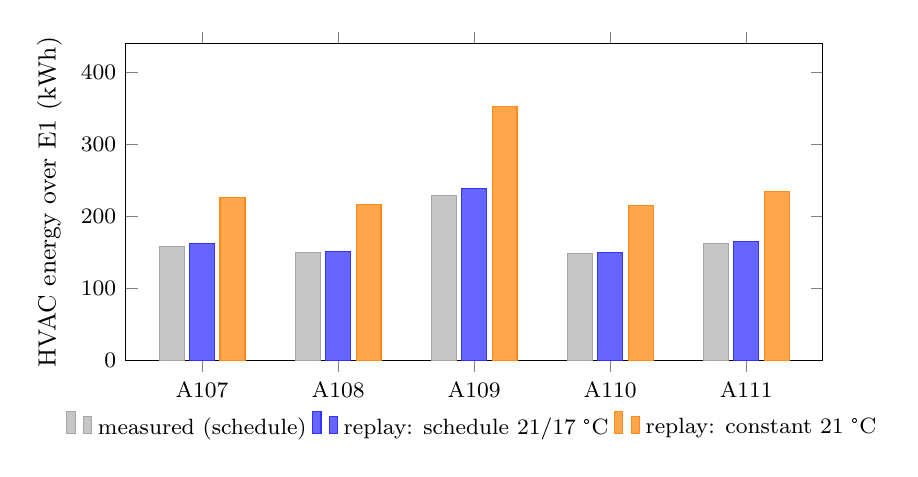
\begin{tikzpicture}
\begin{axis}[ybar, bar width=9pt, width=0.86\linewidth, height=5.6cm, ymin=0, ymax=440,
  ylabel={HVAC energy over E1 (kWh)}, symbolic x coords={A107,A108,A109,A110,A111},
  xtick=data, enlarge x limits=0.14, legend columns=3,
  legend style={font=\footnotesize, draw=none, at={(0.5,-0.14)}, anchor=north},
  tick label style={font=\footnotesize}, label style={font=\small}]
\addplot[fill=gray!45, draw=gray!70] coordinates {(A107,158.5) (A108,149.9) (A109,229.1) (A110,148.7) (A111,162.4)};
\addplot[fill=blue!60, draw=blue!80] coordinates {(A107,163.0) (A108,151.5) (A109,238.3) (A110,150.0) (A111,164.8)};
\addplot[fill=orange!70, draw=orange!90] coordinates {(A107,226.7) (A108,217.2) (A109,352.6) (A110,215.1) (A111,234.5)};
\legend{measured (schedule), replay: schedule 21/17 °C, replay: constant 21 °C}
\end{axis}
\end{tikzpicture}
\caption{HVAC energy over the E1 window per room. The replay feeds E1's measured
occupancy and weather through the production physics and PID code.}
\label{fig:energy}
\end{figure}

\subsection{11.2 CO₂ and occupancy (FR-3, FR-4)}

\begin{figure}[H]
\centering
\begin{tikzpicture}
\begin{groupplot}[group style={group size=1 by 3, vertical sep=0.45cm, xticklabels at=edge bottom},
  width=0.93\linewidth, height=4.3cm, xmin=7.8, xmax=57.1,
  xtick={12,18,24,30,36,42,48,54}, xticklabels={Mon 12:00,Mon 18:00,Tue 00:00,Tue 06:00,Tue 12:00,Tue 18:00,Wed 00:00,Wed 06:00},
  grid=major, grid style={gray!20}, tick label style={font=\footnotesize}, label style={font=\small},
  legend style={font=\footnotesize, draw=none, fill=white, fill opacity=0.85, text opacity=1},
  cycle list name=rooms, no markers]
\nextgroupplot[ylabel={CO$_2$ (ppm)}, ymin=400, ymax=1050, legend columns=5, legend style={at={(0.5,1.03)}, anchor=south}]
\addplot table[x=hour,y=co2_A107,col sep=comma]{data/e1_rooms.csv};
\addplot table[x=hour,y=co2_A108,col sep=comma]{data/e1_rooms.csv};
\addplot table[x=hour,y=co2_A109,col sep=comma]{data/e1_rooms.csv};
\addplot table[x=hour,y=co2_A110,col sep=comma]{data/e1_rooms.csv};
\addplot table[x=hour,y=co2_A111,col sep=comma]{data/e1_rooms.csv};
\addplot[black,dashed] coordinates {(7.8,900) (57.1,900)};
\addplot[red,dashed] coordinates {(7.8,1000) (57.1,1000)};
\legend{A107,A108,A109,A110,A111}
\nextgroupplot[ylabel={Occupants}, ymin=0]
\addplot+[const plot] table[x=hour,y=occ_A107,col sep=comma]{data/e1_rooms.csv};
\addplot+[const plot] table[x=hour,y=occ_A108,col sep=comma]{data/e1_rooms.csv};
\addplot+[const plot] table[x=hour,y=occ_A109,col sep=comma]{data/e1_rooms.csv};
\addplot+[const plot] table[x=hour,y=occ_A110,col sep=comma]{data/e1_rooms.csv};
\addplot+[const plot] table[x=hour,y=occ_A111,col sep=comma]{data/e1_rooms.csv};
\nextgroupplot[ylabel={Ventilation (W)}, xlabel={Simulated time}, ymin=0, ymax=650]
\addplot+[const plot] table[x=hour,y=vent_A107,col sep=comma]{data/e1_rooms.csv};
\addplot+[const plot] table[x=hour,y=vent_A108,col sep=comma]{data/e1_rooms.csv};
\addplot+[const plot] table[x=hour,y=vent_A109,col sep=comma]{data/e1_rooms.csv};
\addplot+[const plot] table[x=hour,y=vent_A110,col sep=comma]{data/e1_rooms.csv};
\addplot+[const plot] table[x=hour,y=vent_A111,col sep=comma]{data/e1_rooms.csv};
\end{groupplot}
\end{tikzpicture}
\caption{E1: CO₂ (dashed lines at the 900 ppm setpoint and the 1000 ppm limit),
head-count from the occupancy simulator, and ventilation command per room.}
\label{fig:co2}
\end{figure}

Five rooms hosted lectures of 24–29 people (Figure~\ref{fig:co2}). CO₂ rose
during each lecture and peaked at 949–966 ppm, just above the 900 ppm setpoint,
where the ventilation loop held it with up to 337 W (median 109 W). In 118 steps a room's
CO₂ was above 900 ppm, and in every one of them the ventilation was on in the next
step, which is the one-step actuation lag of Section 6. No occupied step exceeded
1000 ppm, so FR-3 is met as measured, with a caveat that matters: the rooms are
four times too large (Section 13), which slows the CO₂ rise by the same factor.
With the real volume the replay puts three rooms above 1000 ppm for 7–26 \% of
their occupied steps.

Two behaviours in the figure are model artefacts, not control behaviour. After a
lecture, CO₂ stays where it was, because the CO₂ balance has no infiltration term
and the controller only ventilates above 900 ppm; A110 kept about 880 ppm all
night. And A109's ventilation shows 600 W spikes with no one present: six false
fail-safes, nine steps at full ventilation. A109's true CO₂ sat at 420 ppm for
most of the run, the simulator clamps noisy readings at 420 ppm, so 29 \% of
A109's readings were exactly 420.0, and five identical readings in a row trip the
stuck-sensor rule. The data-quality
check and the sensor model interact in a way neither unit test could show.
FR-4 is met: occupancy reached BuildSim every step, with the lecture blocks
visible in all five rooms.

\subsection{11.3 Cadence and latency (NFR-1)}

Over the nominal part of E1 the simulator stepped every 5.08 s (median;
maximum 5.67 s) and needed 21 ms of work per step for all five rooms (maximum
84 ms). The decision maker made 5808 of the 5810 expected decisions, two per room
per step; the two missing ones are the very first step, before its subscriptions
were in place. Measured on the Docker log clock, a reading took 27 ms from the
simulator's publish to the decision maker (median; 107 ms at p95), and a command
29 ms from decision to confirmed actuator (100 ms at p95), so the whole loop took
59 ms at the median and 207 ms at the 95th percentile, with a worst case of
886 ms (Figure~\ref{fig:latency}). That is five times inside the NFR-1 budget and
1–4 \% of the 5 s step. The tail most likely comes from the sensors opening a new
MQTT connection per message (\texttt{publish.single}) and from the HTTP round
trips to BuildSim inside the sensors and actuators; we did not profile it, because
at this step length it does not matter.

\begin{figure}[H]
\centering
\begin{tikzpicture}
\begin{axis}[width=0.8\linewidth, height=5.6cm, xmin=0, xmax=450, ymin=0, ymax=1,
  xlabel={Latency (ms, real time)}, ylabel={Fraction of decisions},
  grid=major, grid style={gray!20}, legend pos=south east,
  legend style={font=\footnotesize, draw=none}, tick label style={font=\footnotesize}, label style={font=\small}]
\addplot[blue!80!black, thick] table[x=sense_ms,y=q,col sep=comma]{data/e1_latency.csv};
\addplot[orange!90!black, thick] table[x=act_ms,y=q,col sep=comma]{data/e1_latency.csv};
\addplot[black, thick] table[x=total_ms,y=q,col sep=comma]{data/e1_latency.csv};
\legend{simulator $\rightarrow$ decision maker, decision $\rightarrow$ actuator confirmed, total}
\end{axis}
\end{tikzpicture}
\caption{E1: cumulative distribution of per-decision latency over 5808 decisions.
The requirement (NFR-1) is 1000 ms at the 95th percentile.}
\label{fig:latency}
\end{figure}

\subsection{11.4 Fault injection (NFR-2 to NFR-5)}

Each fault was injected into the running E1 stack with Docker commands, one at a
time, with the other four rooms running normally.

\begin{longtable}[]{@{}
  >{\raggedright\arraybackslash}p{(\columnwidth - 6\tabcolsep) * \real{0.22}}
  >{\raggedright\arraybackslash}p{(\columnwidth - 6\tabcolsep) * \real{0.26}}
  >{\raggedright\arraybackslash}p{(\columnwidth - 6\tabcolsep) * \real{0.26}}
  >{\raggedright\arraybackslash}p{(\columnwidth - 6\tabcolsep) * \real{0.26}}@{}}
\toprule
\textbf{Fault} & \textbf{Detection} & \textbf{Behaviour during fault} & \textbf{Recovery} \\
\midrule
\endhead
E2: A110 temperature sensor stopped 65 s & Stale 15.9 s after the last reading (15 s limit + 1 s watchdog tick) & Fail-safe: A110 heating 5.7 kW → 0 W. Other rooms made all 104 expected decisions & PID resumed 0.65 s after the sensor restarted \\
E3: A109 HVAC actuator stopped 44 s & Resend 10.9 s after the first unconfirmed command; 3 resends & A109 heater held its last applied power; other rooms made all 72 expected decisions & Command confirmed 2.5 s after the actuator restarted \\
E4: decision maker killed (SIGKILL) & None: actuators cannot tell & All actuators held their last value; no decisions & Not restarted by Docker; after a manual start, first decision 24 s after the kill \\
E5: MQTT broker stopped 22 s & All 10 loops stale after 15 s & Fail-safe commands undeliverable (actuator resend warnings); simulator crashed 3 times (broker hostname unresolvable) and was restarted & All 10 loops back under control 8.1 s after the broker returned \\
\bottomrule
\end{longtable}

The sensor and actuator faults behaved exactly as designed, including the
isolation: during both outages the other four rooms lost no decisions (NFR-2,
NFR-3, NFR-4). The actuator timeout fired after 10.9 s rather than 10 s because
the watchdog checks once per second and the timeout is strict; the criterion
should have allowed for the tick. The interesting results are E4 and E5. Docker's
\texttt{unless-stopped} policy restarts a container whose process exits, as the
simulator showed three times in E5, but it treats \texttt{docker kill} as a
deliberate stop, so a killed decision maker stays down; a crash would have been
recovered, a kill was not. And in E5 the fail-safe worked on the decision side
but could not reach the actuators: with QoS 0 and no broker, the fail-safe
commands were simply lost, so the actuators held their last values for the 22 s
the broker was gone. That is the right outcome only by luck; a longer outage in
winter would leave heaters running on stale commands. An actuator-side watchdog
(revert to a safe value if no command arrives for a while) is the fix, and is in
Section 13.

\subsection{11.5 Scaling and the breaking point (NFR-6)}

The same procedure (start the stack, wait 150 s after the first step,
measure) was run with 5, 20 and 40 rooms; the five-room run reuses E1's rooms and
larger runs add the next rooms that resolve cleanly (Section 13). Memory is what
limits the design (Figure~\ref{fig:scale}). Each controlled room adds five
Python containers of about 19 MiB each as Docker reports them, but the VM's used
memory grows by 116 MiB per room, 23 MiB per container once
the runtime's per-container overhead is included. At 40 rooms the stack ran 208
containers in 5966 MiB of the VM's 7789 MiB, with no
restarts and no missed decisions; the linear fit reaches the VM's memory at about
56 rooms.

Latency sets a similar limit. The shared simulator's work per step grew from
27 ms to 253 ms, harmless
against a 5 s step, but the 95th percentile of the whole loop grew from
123 ms to 704 ms, by about 21 ms per
room between 20 and 40 rooms, which would cross NFR-1's 1 s budget near
54 rooms. Both halves of the loop slow down (at the median, sensing from
108 to 319 ms and actuation from 70 to 218 ms between 20 and 40 rooms), which
points at per-message work that serialises the burst of 2N messages each step
produces: every hop makes an HTTP call to BuildSim, and the decision maker handles
messages one at a time, calling the occupancy simulator for every temperature
reading to look up the setpoint. We did not profile which dominates; caching the
setpoint once per step is the cheap first fix.

The projection for the earlier design (eight containers per room, no shared
services) shows why consolidation was necessary but not sufficient. It would fill
the VM at about 35 rooms, and its 952 containers for all 119 configured
rooms would need about 23 GB, so it could not have run on this laptop even
with the occupancy simulator's health check fixed. The current design runs 40
rooms comfortably but would still need about 11 GB for the 84 rooms that
resolve cleanly: one container per emulated device is right for demonstrating
fault isolation and wrong for a whole building.

The 40-room run also found an operational limit. With 202 services sharing one
build section, \texttt{docker compose up --build} failed inside BuildKit (``no such
job''); building the shared image once and then starting with \texttt{up -d}
works, and \file{run\_scale.sh} now does that.

\begin{figure}[H]
\centering
\begin{tikzpicture}
\begin{axis}[width=0.86\linewidth, height=6.2cm, xmin=0, xmax=70, ymin=0, ymax=8500,
  xlabel={Controlled rooms}, ylabel={Docker VM memory used (MiB)},
  grid=major, grid style={gray!20}, legend pos=south east,
  legend style={font=\footnotesize, draw=none, fill=white, fill opacity=0.85, text opacity=1},
  tick label style={font=\footnotesize}, label style={font=\small}]
\addplot[blue!80!black, thick, mark=*] table[x=rooms,y=vm_used_MiB,col sep=comma]{data/scale.csv};
\addplot[blue!80!black, dashed, domain=0:70] {1326+115.9*x};
\addplot[orange!90!black, dashed, domain=0:70] {1280+185.4*x};
\addplot[red, thick] coordinates {(0,7789) (70,7789)};
\legend{measured (5 containers per room), fit: current design, projected: 8 containers per room, VM memory (7789 MiB)}
\end{axis}
\end{tikzpicture}
\caption{Memory used in the Docker VM against the number of controlled rooms,
measured 150 s after the first simulation step, with a linear fit and the
projection for the earlier design with per-room simulator and decision makers.}
\label{fig:scale}
\end{figure}

\textbf{Per-run measurements.} Each row is one run of \file{run\_scale.sh},
measured 150 s (about 30 steps) after the first simulation step; the decisions
column excludes each run's first and last step.

\begin{longtable}[]{@{}
  >{\raggedleft\arraybackslash}p{(\columnwidth - 12\tabcolsep) * \real{0.09}}
  >{\raggedleft\arraybackslash}p{(\columnwidth - 12\tabcolsep) * \real{0.13}}
  >{\raggedleft\arraybackslash}p{(\columnwidth - 12\tabcolsep) * \real{0.14}}
  >{\raggedleft\arraybackslash}p{(\columnwidth - 12\tabcolsep) * \real{0.17}}
  >{\raggedleft\arraybackslash}p{(\columnwidth - 12\tabcolsep) * \real{0.17}}
  >{\raggedleft\arraybackslash}p{(\columnwidth - 12\tabcolsep) * \real{0.18}}
  >{\raggedleft\arraybackslash}p{(\columnwidth - 12\tabcolsep) * \real{0.12}}@{}}
\toprule
\textbf{Rooms} & \textbf{Containers running} & \textbf{VM memory used (MiB)} & \textbf{Simulator work per step, p50 / max (ms)} & \textbf{Latency p50 / p95 (ms)} & \textbf{Decisions missed / expected} & \textbf{Restarts} \\
\midrule
\endhead
5 & 33 & 1911 & 27 / 71 & 63 / 123 & 0 / 290 & 0 \\
20 & 108 & 3634 & 111 / 166 & 193 / 280 & 4 / 1160 & 0 \\
40 & 208 & 5966 & 253 / 429 & 571 / 704 & 0 / 2320 & 0 \\
\bottomrule
\end{longtable}

\subsection{11.6 Results against the requirements}

\begin{longtable}[]{@{}
  >{\raggedright\arraybackslash}p{(\columnwidth - 6\tabcolsep) * \real{0.10}}
  >{\raggedright\arraybackslash}p{(\columnwidth - 6\tabcolsep) * \real{0.34}}
  >{\raggedright\arraybackslash}p{(\columnwidth - 6\tabcolsep) * \real{0.42}}
  >{\raggedright\arraybackslash}p{(\columnwidth - 6\tabcolsep) * \real{0.14}}@{}}
\toprule
\textbf{Req.} & \textbf{Criterion} & \textbf{Measured} & \textbf{Verdict} \\
\midrule
\endhead
FR-1 & Reach 21 °C in 24 h, then ±1 °C (T-1); live: ≥ 90 \% of daytime steps in band & T-1 passes. Live: 35–63 \% of daytime and 52 \% of occupied steps in band; mornings need 2.4–6.3 h & ✗ live \\
FR-2 & Switch within one step; less energy than constant 21 °C & All four switches in the first step; 30 \% less HVAC energy (replay), at a large comfort cost & ✓ \\
FR-3 & Ventilation on above 900 ppm; full room below 1000 ppm in 10 min & On in the next step in 118 of 118 cases; no occupied step above 1000 ppm (peak 966); T-2 passes & ✓\textsuperscript{c} \\
FR-4 & Head-count in BuildSim every step & Every step; lectures of 24–29 people in all rooms; T-3 passes & ✓ \\
FR-5 & Rooms chosen by flag only & 5, 20 and 40 rooms deployed by flag and generator; T-7 & ✓ \\
NFR-1 & Every room every step; p95 < 1 s & 5808 of 5810 decisions; p95 207 ms at 5 rooms, 704 ms at 40 & ✓ \\
NFR-2 & Fail-safe within 1 s of the 15 s limit; resume on good data & 15.9 s; resumed 0.65 s after the sensor returned; but six false stuck alarms in E1 & ✓\textsuperscript{c} \\
NFR-3 & Detect within 10 s; resend until confirmed & 10.9 s (1 s watchdog tick); 3 resends; confirmed 2.5 s after restart & ≈ \\
NFR-4 & Other rooms unaffected & All 104 and 72 expected decisions made during E2 and E3; T-6 & ✓ \\
NFR-5 & Control back within 60 s, no manual action & Broker outage: 8.1 s. Killed decision maker: not restarted by Docker & ✗ \\
NFR-6 & 5 rooms < 2 GB; ≥ 20 rooms in 8 GB & 5 rooms: 1911 MiB in the VM; 40 rooms: 5966 MiB; limit about 55 rooms & ✓ \\
\bottomrule
\end{longtable}

{\footnotesize \textsuperscript{c} Met as measured, with the caveat given in the text (FR-3: rooms four times too large; NFR-2: false alarms).\par}

Eight of the eleven requirements are met as measured, two of them with a caveat;
NFR-3 is missed by the watchdog's one-second tick; FR-1 fails in the live system
and NFR-5 fails for a killed decision maker. The failures share a pattern worth
stating plainly: every component passed its unit test, and every failure appeared
only when the whole system ran for long enough, with real occupancy, a real
schedule and real faults. That is the strongest argument this project produced
for end-to-end evaluation, and the reason Section 13 is longer than we expected.

%% ===========================================================================
\section{12. Dashboard}

The dashboard is a Grafana board provisioned from \file{monitoring/} when the
stack starts, so it needs no manual setup and lives in version control. It shows
the outside temperature, the occupancy simulator's clock in Swedish time, and six
per-room time series: temperature, setpoint, HVAC power, CO₂, ventilation command
and occupancy. A room selector filters the room panels, and the board refreshes
every 5 s real, once per simulated step. BuildSim's own 3D viewer, open next to it,
shows the same sensor values on the rooms and the occupancy simulator's people
moving; the two views share a source of truth, so they cannot disagree.

\begin{figure}[H]
\centering
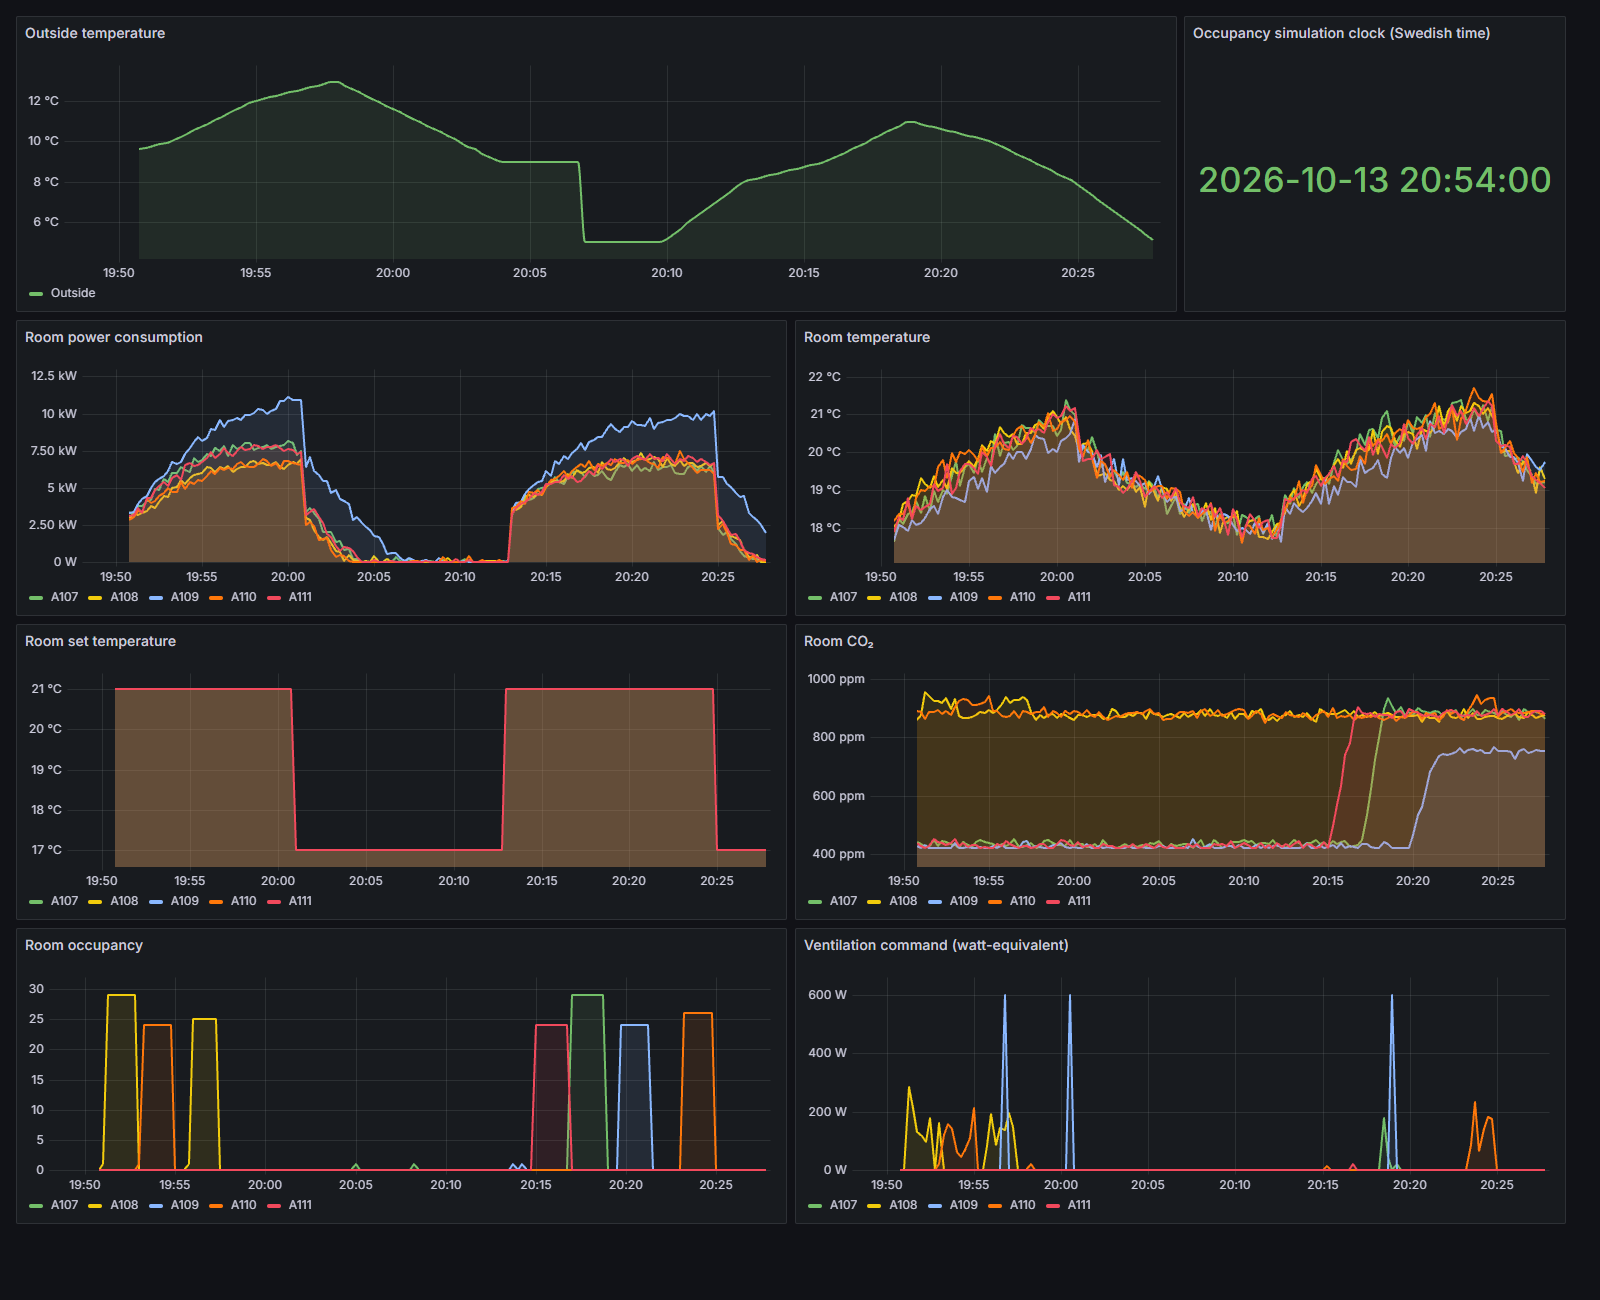
\includegraphics[width=\textwidth]{figures/dashboard-grafana.png}
\caption{The dashboard at the end of E1's nominal window, captured headless from
the running stack. The x-axis is real time (37 real minutes, about 37 simulated
hours); the clock panel shows the simulated time.}
\label{fig:dashboard}
\end{figure}

The screenshot tells the E1 story at a glance: the setpoint panel shows the
21/17 °C schedule, the power panel the heating ramping up on two mornings,
halving at 18:00 and winding down over the evening, the occupancy panel the
lectures arriving in different rooms each day, and the CO₂ panel rooms rising
during lectures and then staying at the new level. The ventilation panel also shows something we
did not intend: 600 W spikes in A109 with no one in the room. They are false
fail-safes, explained in Section 11.4; the dashboard is how we found them.

What the dashboard does not show is the decision maker's internal state: whether a
loop is in fail-safe or waiting for an acknowledgement is visible only in the
container log. That is the first thing we would add (Section 13).

%% ===========================================================================
\section{13. Risks and critical reflection}

Writing the evaluation found more problems than building the system did, and
the most useful ones are below, worst first. None of them was visible from the
unit tests alone; they came from running the whole stack and reading the
numbers.

\textbf{1. The rooms are four times too large.} BuildSim reports room
\texttt{area} in plan units² (0.25 m² each at the occupancy simulator's
0.5 m per unit), and \file{con-sim.py} uses that number as m². A107 is
122 m² to the occupancy simulator but 490 ``m²'' to our physics, so every room's
air volume, thermal mass and envelope are four times too large. This one bug
explains two results that looked like design properties: the slow warm-up
(Section 11.1) and the comfortable CO₂ margin (Section 11.2). Replaying E1 with
the area corrected, the same controller reaches 20.5 °C in 0.7–3.8 h instead
of 5.4–10.1 h, but A108's CO₂ peaks at 1019 ppm and is above
1000 ppm for 15 \% (A107: 26 \%) of its occupied steps: the ventilation gains that
look adequate today are too weak for a real lecture room. Fixing the conversion
is one line; retuning the CO₂ loop is the follow-up it forces.

\textbf{2. The simulator stops every simulated weekend.} \file{Weather.json}
covers Monday to Friday only, and the outside-temperature lookup sits outside the
per-room error handling, so on Saturday the simulator raises, Docker restarts it,
and it raises again at the first step. At factor 60 that happens 1.9 real hours
after a Monday 07:30 start and lasts 48 real minutes. The decision maker then
correctly fails safe in every room, so the building is not harmed, but no physics
runs. Either the data or a fallback (repeat Friday) is needed before a long demo.

\textbf{3. The controller integrates real time, the plant simulated time.} The PID
uses \texttt{time.monotonic()}, so $K_i$ and $K_d$ are effectively per real
second, while the plant evolves 60 times faster. The gains are therefore only
valid at factor 60: at factor 120 the integral action per simulated hour halves.
Readings should carry the simulated timestamp, and the PID should use it. A
related detail showed up at every 18:00: the integral is not reset when the
setpoint drops, so the heating takes 2–6 hours to wind down instead of stopping.

\textbf{4. The schedule ignores both occupancy and thermal lag.} The 06:00
setpoint step reaches the rooms only after 2.4–6.3 hours (Section 11.1), so
lectures at 08:15 start below the comfort band, while four of the five rooms sat
empty for most of the day and were heated anyway. The setback saved
30 \% of the HVAC energy against a constant 21 °C; an occupancy-aware setback with an
optimal-start ramp (start heating early enough to reach 21 °C when the first
lecture begins) would address both the comfort miss and the remaining waste, and
is the main improvement to the autonomous part.

\textbf{5. CO₂ never decays without mechanical ventilation.} The CO₂ balance has no
infiltration term, although the heat balance does ($\text{ACH}_0 = 0.5$
h$^{-1}$). An empty room therefore keeps its last CO₂ value until the damper
opens, which is why A110 sat at about 870 ppm overnight. Adding the same
background air change to the CO₂ balance fixes it.

\textbf{6. The stuck-sensor rule raises false alarms.} Five identical readings
mean ``stuck'' only if a live sensor never repeats itself. Our simulated CO₂
sensor does repeat itself whenever the true value is at the 420 ppm floor, because
noise below the floor is clamped, and A109 failed safe six times with nobody in
the room (Section 11.2). It is systematic, not a one-off: in the 20-room scaling
run, newly enabled rooms start at the 420 ppm default and seven of the fifteen
raised the same false alarm within 2.5 minutes. The cost per alarm is small (a
step or two of full ventilation), but the lesson is general: a data-quality rule encodes an assumption about the
sensor, and here the sensor model broke it. The rule should ignore readings at a
physical bound, or the simulator should not clamp.

\textbf{7. The shared services are single points of failure.} Consolidation (D2,
D3) traded per-room isolation for a system that starts. We mitigated rather than
removed the risk: in-process isolation, a restart policy and the fail-safe.
E4 and E5 show what is left: killing the decision maker left every actuator at its last value, and Docker did not restart a container it had killed itself, so control came back only after a manual start (24 s after the kill, 20 s of which was our wait). The broker outage needed no help: all loops resumed 8 s after the broker returned, although the simulator crashed and restarted three times while it was gone. The same consolidation has a subtler
cost: the shared simulator refuses to start if any enabled room is missing from
BuildSim and waits indefinitely for any room whose devices never register, so one
misconfigured room now stops the physics for all of them. And 20 of the 119 rooms
in \file{rooms.json} have no unique match in the occupancy simulator; enabling all
rooms today would crash those rooms' occupancy publishers in a loop. The generator
should validate rooms before writing the compose file.

\textbf{8. The fail-safe needs the broker it is protecting against.} The decision
maker decides to fail safe, but the actuators only hear it over MQTT. In E5 the
broker was the failure, so the fail-safe commands were lost and the actuators held
their last values for 22 s. A watchdog in each actuator (revert to a safe value
when no command has arrived for, say, three steps) would make the fail-safe
independent of the network, which is where a real BMS puts it.

\textbf{9. Per-device containers cost memory.} Each Python container takes about
23 MiB of VM memory including Docker's overhead, so five devices per room dominate
the footprint. The measured breaking point (Section 11.5) is about 55 rooms on
this laptop, where the 8 GB VM fills up and the loop latency reaches its 1 s
budget at roughly the same point. The device-per-container
principle is right for a demonstration of fault isolation; a real deployment would
run many virtual devices per process, or real devices.

\textbf{10. The fail-safe for heating is ``off''.} That is safe against a frozen
reading driving the heater, but a long sensor outage in winter cools the room
without bound. A frost-protection minimum instead of 0 W would be the better
default for a real building.

\textbf{11. Monitoring has no memory and no view of decisions.} Prometheus stores
to tmpfs, so a restart erases the evaluation data unless it is exported first (we
exported ours), and the dashboard cannot show whether a loop is in fail-safe or
retrying. Exporting the controller state as metrics would be a small change with a
large effect on trust.

\textbf{12. No authentication anywhere.} MQTT accepts anonymous clients and
BuildSim has no authentication. Publishing every port only on 127.0.0.1 keeps this
acceptable on a laptop, but any process on the machine can command an actuator.

\begin{longtable}[]{@{}
  >{\raggedright\arraybackslash}p{(\columnwidth - 4\tabcolsep) * \real{0.34}}
  >{\raggedright\arraybackslash}p{(\columnwidth - 4\tabcolsep) * \real{0.26}}
  >{\raggedright\arraybackslash}p{(\columnwidth - 4\tabcolsep) * \real{0.40}}@{}}
\toprule
\textbf{Risk / assumption} & \textbf{Impact} & \textbf{Mitigation / next step} \\
\midrule
\endhead
Area in plan units used as m² & Wrong dynamics; CO₂ loop under-tuned & Convert ×0.25; retune ventilation gains \\
No weekend weather data & No physics 48 h per simulated week & Add data or repeat Friday; catch the error per step \\
PID on real time & Gains tied to factor 60 & Use simulated timestamps in readings \\
Clock-only setback & Cold mornings, heated empty rooms & Occupancy-aware setback with optimal start \\
Stuck rule meets clamped sensor & False fail-safes (6 in E1) & Ignore readings at a physical bound \\
Shared \texttt{dec}/\texttt{sim} & All rooms affected by one crash; \texttt{kill} not restarted & Restart policy covers crashes (E5); external health check for the rest \\
Fail-safe travels over MQTT & Lost when the broker is down (E5) & Actuator-side watchdog; QoS 1 for commands \\
Five containers per room & Memory caps the room count & Several devices per process beyond a demo \\
Unvalidated \file{rooms.json} & Crash loops for 20 of 119 rooms & Validate against BuildSim and occupancy simulator in the generator \\
\bottomrule
\end{longtable}

\textbf{What we would do next}, in order: fix the area conversion and retune the
CO₂ loop; make the simulator survive weekends and broker outages; feed simulated
time to the PID and reset its integral on setpoint changes; stop clamping the
simulated CO₂ sensor; add a watchdog in each actuator; replace the clock setback
by an occupancy-aware optimal start; export controller state to the dashboard.
The first four are bugs that the evaluation found; the last three are the design
work that would make the autonomous part genuinely better.

\end{document}
